\documentclass[10pt,twocolumn,letterpaper]{article}

\usepackage{graphicx}
\usepackage{amsmath}
\usepackage{amssymb}
\usepackage{booktabs}
\usepackage[table,xcdraw]{xcolor}
\usepackage{listings}
\usepackage{pgfplots}
\usepackage{pgfplotstable}
\usepackage{tikz}
\usetikzlibrary{positioning}
\usepackage{subcaption}
\usepackage{url}
\usepackage[numbers]{natbib}
\usepackage{hyperref}
\usepackage[capitalize]{cleveref}

\pgfplotsset{compat=1.18}

\lstset{
  basicstyle=\ttfamily\footnotesize,
  breaklines=true,
  frame=single,
  language=C,
  keywordstyle=\bfseries,
  commentstyle=\itshape,
  showstringspaces=false
}

\begin{document}

\title{SqC: A Tree-Sitter Based Static Analyzer for\\CERT C Coding Standard Compliance}

\author{Brandon Arrendondo\\
{\tt\small brandon.arrendondo@bissell.com}
\and
Eric Buehler\\
{\tt\small eric.buehler@bissell.com}
\and
Tristan Vanfossen\\
{\tt\small tristan.vanfossen@bissell.com}
}
\maketitle

\begin{abstract}
Static analyzers for C either check a narrow subset of vulnerability
classes or require the build infrastructure---a compiler, a compilation
database, a preprocessing pass---that the code most in need of checking
does not yet have.  This paper asks how far a source-only analyzer can
be pushed instead, and answers with SqC, which checks C against 311
rules of the SEI CERT C Coding Standard from tree-sitter parse trees
alone: no compiler, no build system, no compilation database, and
tolerant of source that does not compile.  On that foundation SqC
constructs per-function control-flow graphs, forward null-state
dataflow, value-range analysis, and inter-procedural function summaries
with cross-function taint propagation.

We evaluate at two levels.  On the NIST Juliet Test Suite v1.3 (50,256
files, 79 CWE categories), precision reaches 87.1\% with 43 of 79 CWEs
at 100\%.  On nine real-world open-source codebases (1.21 million
lines), a human-adjudicated oracle gives 24.3\% precision at 93.7\%
recall against known true positives---a very different picture, and the
paper's second contribution is why the two disagree.  A presence-based
synthetic oracle scores whether a defect was found; it cannot see an
analyzer that emits one finding a hundred times, so whole classes of
misbehavior are invisible to Juliet by construction.

Detection breadth remains the binding constraint: SqC flags 12.9\% of
Juliet's planted flaw lines, and 40\% of its 311 rules have no
true-positive evidence on either corpus---a limit of the corpora as
much as of the tool, since both are compilable, warning-clean code and
SqC's target population is neither.  Against cppcheck, clang-tidy,
Infer and Frama-C, SqC covers 5--13$\times$ more CWE categories,
implementing 311 CERT C rules where cppcheck and clang-tidy implement
roughly 20 each: breadth and deployment independence bought at a
measured cost in per-CWE depth.
\end{abstract}


%% ============================================================
\section{Introduction}
\label{sec:intro}

The C programming language remains dominant in systems software,
embedded systems, and security-critical infrastructure.  Despite decades
of research in programming language safety, C's lack of memory safety
guarantees continues to produce vulnerabilities: buffer overflows, null
pointer dereferences, integer overflows, and use-after-free defects
account for the majority of CVEs in C codebases~\cite{cwe-top25}.

The SEI CERT C Coding Standard~\cite{cert-c} codifies 120+ rules and
200+ recommendations spanning 17 categories, from integer handling to
concurrency to POSIX-specific interfaces.  While the standard is widely
referenced in secure coding guidelines (e.g., MISRA C, IEC 62443),
tool support for comprehensive CERT C checking remains fragmented.
Commercial tools such as Coverity~\cite{coverity}, Klocwork, and
Polyspace implement subsets of CERT C rules alongside proprietary
checkers, but their closed-source nature limits reproducibility.
Open-source alternatives like cppcheck~\cite{cppcheck} and
clang-tidy~\cite{clang-tidy} implement approximately 20 CERT C checks
each, leaving the majority of the standard uncovered.

This paper presents SqC (\textbf{S}oftware Code \textbf{Q}uality for
\textbf{C}), a static analysis tool that implements 311 CERT C rules
across all 17 categories.  The paper describes the tool's architecture,
the iterative process used to reduce false positives, and the results of
evaluating SqC against both a standardized benchmark and real-world
codebases.

The rest of this paper is organized as follows.  \Cref{sec:background}
covers the CERT C standard and the Juliet benchmark.
\Cref{sec:architecture} describes SqC's architecture.
\Cref{sec:methodology} details the testing methodology.
\Cref{sec:results} presents benchmark results.
\Cref{sec:fp-reduction} walks through the iterative false positive
reduction process.  \Cref{sec:worked-example} provides a worked
example.  \Cref{sec:limitations} discusses limitations.
\Cref{sec:related} covers related work.  \Cref{sec:conclusion}
concludes.


%% ============================================================
\section{Background}
\label{sec:background}

\subsection{SEI CERT C Coding Standard}

The SEI CERT C Coding Standard is maintained by the Software
Engineering Institute at Carnegie Mellon University.  It defines rules
and recommendations organized into 17 categories, shown in
\cref{tab:cert-categories}.

\begin{table}[t]
\centering
\footnotesize
\begin{tabular}{@{}llr@{}}
\toprule
\textbf{Prefix} & \textbf{Category} & \textbf{Rules} \\
\midrule
API & API Usage & 9 \\
ARR & Arrays & 9 \\
CON & Concurrency & 23 \\
DCL & Declarations & 32 \\
ENV & Environment & 9 \\
ERR & Error Handling & 11 \\
EXP & Expressions & 31 \\
FIO & File I/O & 35 \\
FLP & Floating Point & 14 \\
INT & Integers & 23 \\
MEM & Memory Mgmt & 17 \\
MSC & Miscellaneous & 31 \\
POS & POSIX & 21 \\
PRE & Preprocessor & 16 \\
SIG & Signals & 7 \\
STR & Strings & 16 \\
WIN & Windows & 7 \\
\midrule
& \textbf{Total} & \textbf{311}\textsuperscript{$\dagger$} \\
\bottomrule
\end{tabular}
\caption{CERT C rule categories implemented in SqC.
\textsuperscript{$\dagger$}Includes both mandatory rules and advisory
recommendations.}
\label{tab:cert-categories}
\end{table}

Each rule addresses a specific class of undefined behavior, security
vulnerability, or quality defect.  For example, EXP34-C (``Do not
dereference null pointers'') maps directly to CWE-476; INT32-C
(``Ensure that operations on signed integers do not result in
overflow'') maps to CWE-190.  The standard provides a rule-to-CWE
mapping that enables systematic benchmarking.

\subsection{NIST Juliet Test Suite}

The Juliet Test Suite v1.3~\cite{juliet} (commit \texttt{f88433e})
is developed by NIST's
Software Assurance Metrics and Tool Evaluation (SAMATE) project.
It contains 64,099 C/C++ test cases across 118 CWE categories,
organized into ``good'' functions (correct code that should not
trigger warnings) and ``bad'' functions (code containing the
specified vulnerability).

Juliet provides a controlled evaluation environment: each test case
isolates a single vulnerability type with known ground truth, enabling
precise measurement of true positive (TP) and false positive (FP) rates
per CWE.

Juliet also has known limitations worth acknowledging.  Test cases use
synthetic patterns that may not reflect real-world coding idioms.  The
structured naming conventions (functions prefixed with \texttt{bad} or
\texttt{good}) can inadvertently advantage or disadvantage
pattern-matching tools.  And Juliet uses explicit C types
(\texttt{int}, \texttt{unsigned int}) rather than \texttt{stdint.h}
typedefs (\texttt{uint32\_t}), so fixes targeting typedef resolution
show impact on real-world code but not on Juliet.

These limitations are why we supplement Juliet with real-world
evaluation.

\subsection{Real-World Benchmarks}

Nine open-source C projects serve as real-world benchmarks:
libcrc (1K LOC), lua (31K LOC), raylib (56K LOC), mosquitto (39K LOC),
curl (186K LOC), sqlite (182K LOC), hostap (590K LOC), pure-ftpd (33K
LOC), and seL4 (87K LOC).  These span embedded libraries,
scripting-language runtimes, game/graphics libraries, network servers,
databases, an FTP daemon, and a formally verified microkernel.  Lua and
raylib were added as a fifth and sixth ground-truth oracle specifically
to exercise C99 idioms (compound literals, designated initializers) that
the original five-project set does not contain (\cref{sec:sloc-scope});
pure-ftpd was added as an eighth oracle to exercise SQL-client-API call
sites (\texttt{mysql\_real\_query}, \texttt{PQexec}) absent from the
other codebases, and seL4 as a ninth to test a freestanding,
formally-verified, hardware-facing codebase with no libc/POSIX surface.


%% ============================================================
\section{Architecture}
\label{sec:architecture}

SqC is implemented in Rust (2021 edition) and uses tree-sitter for
parsing.  The analysis pipeline proceeds in four stages, illustrated
in \cref{fig:pipeline}.

\begin{figure}[t]
\centering
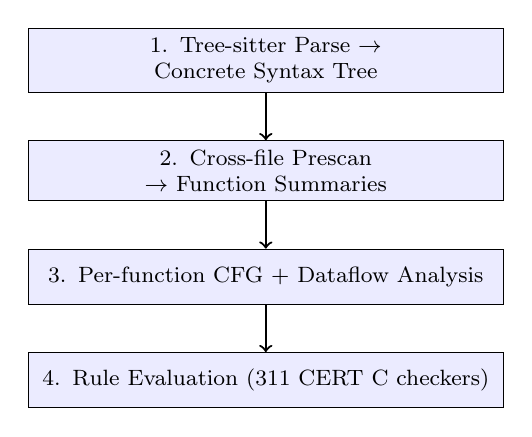
\begin{tikzpicture}[
    node distance=0.6cm,
    box/.style={rectangle, draw, fill=blue!8, text width=5.8cm,
                minimum height=0.7cm, align=center, font=\footnotesize},
    arrow/.style={->, thick}
]
\node[box] (parse) {1. Tree-sitter Parse $\rightarrow$ Concrete Syntax Tree};
\node[box, below=of parse] (prescan) {2. Cross-file Prescan $\rightarrow$ Function Summaries};
\node[box, below=of prescan] (cfg) {3. Per-function CFG + Dataflow Analysis};
\node[box, below=of cfg] (rules) {4. Rule Evaluation (311 CERT C checkers)};
\draw[arrow] (parse) -- (prescan);
\draw[arrow] (prescan) -- (cfg);
\draw[arrow] (cfg) -- (rules);
\end{tikzpicture}
\caption{SqC analysis pipeline.  Each stage enriches the context
available to subsequent stages.}
\label{fig:pipeline}
\end{figure}

\subsection{Stage 1: Parsing with Tree-sitter}

SqC uses tree-sitter~\cite{tree-sitter} to produce a concrete syntax
tree (CST) for each C source file.  Unlike tools built on Clang's AST
(which requires a full compilation database), tree-sitter operates on
individual files without preprocessing.  This trades semantic precision
for practical deployability: SqC can analyze any C file without build
system integration.

The primary limitation is the inability to resolve preprocessor macros
and \texttt{\#include} directives.  SqC mitigates this through a
built-in database of approximately 370 standard library and platform
API functions (\cref{sec:stdlib-db}).

\subsection{Stage 2: Cross-File Prescan}
\label{sec:prescan}

When invoked with the \texttt{-d} (directory) flag, SqC performs a
pre-scan pass over all C files in the specified directories, collecting:

\begin{itemize}
    \item \textbf{Function definitions}: name, file, parameter count,
        and return type.
    \item \textbf{Function summaries}: per-parameter null state
        (DefinitelyNull, PossiblyNull, NotNull, Unknown) derived from
        call-site argument analysis across the project.
    \item \textbf{Local variable states}: within each function body,
        assignments to local variables are tracked to resolve argument
        values passed at call sites.
\end{itemize}

This was the single largest contributor to false positive reduction,
removing 148,622 FPs (31.2\%) in one iteration (\cref{sec:fp-cross-file}).

\subsection{Stage 3: Control-Flow Graphs and Dataflow}

For each function, SqC constructs a control-flow graph (CFG) handling
\texttt{if}/\texttt{else}, \texttt{switch}/\texttt{case}, loops with
\texttt{break}/\texttt{continue}, early returns, and \texttt{goto}
statements.

On the CFG, SqC performs forward dataflow analysis for null pointer
state tracking.  The null state lattice is:

\begin{equation}
\text{NullState} \in \{\text{Unknown}, \text{DefinitelyNull},
    \text{PossiblyNull}, \text{NotNull}\}
\end{equation}

Edge refinement propagates null information through branch conditions:
after \texttt{if (p != NULL)}, the true branch marks \texttt{p} as
NotNull while the false branch marks it as PossiblyNull.

The CFG infrastructure also supports:
\begin{itemize}
    \item A \textbf{constant evaluator} that resolves \texttt{sizeof}
        expressions, C standard limit macros (\texttt{INT\_MAX},
        \texttt{UINT64\_MAX}), file-scope \texttt{static const int}
        declarations, and compile-time arithmetic.
    \item \textbf{Dead-branch pruning}: when a branch condition
        resolves to a compile-time constant (literal, \texttt{\#define},
        or \texttt{static const}), only the feasible branch is included
        in the CFG, improving precision for all downstream analyses.
    \item \textbf{Initialization state tracking} for detecting
        use of uninitialized variables through conditional paths.
    \item \textbf{Value-range analysis} (VRA) for integer and
        floating-point overflow rules, tracking variable ranges through
        assignments, branches, and loop bounds.
\end{itemize}

\subsection{Stage 4: Rule Evaluation}

Each of the 311 rules is implemented as a Rust struct implementing
the \texttt{CertRule} trait.  Rules range from simple AST pattern
matchers (e.g., MSC24-C: obsolete function detection) to complex
multi-pass analyzers (e.g., EXP34-C: null dereference detection
using CFG-based dataflow with inter-procedural call-site propagation).

\textbf{UTF-8 source encoding.}  Tree-sitter represents all source
positions as byte offsets into the raw UTF-8 source file.  Industrial
C codebases routinely embed non-ASCII content in comments and string
literals: comments written in Chinese, Japanese, Arabic, Cyrillic, or
other scripts are common in embedded and international software
projects.  Rule implementations that inspect raw source text must
therefore use byte-indexed string operations throughout.
Character-counted indices produce incorrect slices---or runtime panics
in languages with strict Unicode safety---when a multi-byte sequence
falls before a slice boundary.  For example, a Chinese full-width
parenthesis (\texttt{U+FF08}, three UTF-8 bytes) encountered during
real-world analysis triggered a panic in the ARR00-C and PRE02-C
checkers, both of which were using \texttt{chars().enumerate()} indices
(character positions) as byte offsets.  SqC enforces the requirement
for byte-safe slicing through \texttt{char\_indices()}-based iteration
and includes UTF-8 regression test cases in each affected rule's test
suite.

\subsection{Standard Function Database}
\label{sec:stdlib-db}

Since tree-sitter cannot follow \texttt{\#include} directives, SqC
maintains a built-in database of approximately 370 known functions:
$\sim$180 C11 standard library, $\sim$90 POSIX, and $\sim$100 Windows
API functions.  This database serves multiple purposes: DCL31-C/DCL07-C
use it to avoid flagging standard library calls as undeclared; ERR33-C
uses it to identify functions whose return values must be checked;
EXP10-C uses a pure-function whitelist to exclude side-effect-free
calls from unsequenced evaluation warnings.


%% ============================================================
\section{Testing Methodology}
\label{sec:methodology}

\subsection{Juliet Benchmark Protocol}

The Juliet benchmark operates in two modes:

\textbf{Full mode}: All 305 enabled rules are applied to all 118 CWEs.  This
measures overall tool behavior but introduces noise from rules
triggering on CWEs they were not designed to detect.

\textbf{Fast mode}: Per-CWE rule manifests restrict each scan to only
the CERT C rules mapped to that CWE.  A mapping script generates 147
TOML manifest files from the official CERT C rule-to-CWE mapping.
This eliminates cross-CWE noise and reduces scan time by approximately
10$\times$.  All results from v0.3.20 onward use fast mode.

For each CWE directory, the benchmark invokes SqC with cross-file
analysis enabled, then classifies each violation by file name:
violations in \texttt{*bad*} files are True Positives; violations in
\texttt{*good*} files are False Positives.  Results are stored in a
SQLite database with per-violation granularity.

\textbf{TP rate} is defined as $\frac{\text{TP}}{\text{TP}+\text{FP}}$
(precision), not recall.  A ``bad'' file may contain multiple violation
types, but only the intended CWE is scored as TP.

\subsection{Real-World Benchmark Protocol}

Seven open-source C projects (\cref{tab:realworld-codebases}) are
analyzed with SqC, cppcheck (v2.10), and clang-tidy (v21.1.6).

\begin{table}[t]
\centering
\footnotesize
\begin{tabular}{@{}lrrl@{}}
\toprule
\textbf{Project} & \textbf{C Files} & \textbf{LOC} & \textbf{Commit} \\
\midrule
libcrc & 9 & 1,034 & \texttt{7719e21} \\
lua & 33 & 31,637 & \texttt{40b76de2} \\
raylib & 17 & 56,107 & \texttt{962bbfc} \\
mosquitto & 120 & 39,368 & \texttt{d3ee5c5} \\
curl & 222 & 186,220 & \texttt{3e198f75} \\
sqlite & 125 & 218,733 & \texttt{b1a73ba34} \\
hostap & 430 & 589,724 & \texttt{dcee6043} \\
\midrule
\textbf{Total} & \textbf{956} & \textbf{1,122,823} & \\
\bottomrule
\end{tabular}
\caption{Real-world benchmark codebases.}
\label{tab:realworld-codebases}
\end{table}

Real-world analysis revealed robustness requirements absent from the
Juliet benchmark.  Industrial embedded codebases frequently contain
comments written in non-Latin scripts: running SqC against a battery
management system codebase with Chinese-language function comments
uncovered a latent crash in three rule checkers caused by unsafe
UTF-8 string slicing (\cref{sec:architecture}).  The benchmark suite
itself later exposed two more analyzer-crashing defect classes that
Juliet never exercises.  hostapd's configuration parser contains an
\texttt{else if} chain several thousand branches deep, which overflowed
the stack in every rule checker that walked the AST by self-recursion
(three checkers crashed before the recursive walks were converted to
explicit-stack iteration); and a curl unit test containing a string
literal with a \texttt{]} character preceding the \texttt{[} of an
array subscript triggered an out-of-bounds slice in a bounds-checking
rule.  Juliet's test cases are structurally simple ASCII programs, so
none of these defect classes---encoding, nesting depth, or adversarial
token ordering---are visible to benchmark-only validation; all of them
surfaced exclusively through real-world analysis.

These experiences motivated a methodological decision: the real-world
suite is run under the same protocol rigor as Juliet.  Every run is
tied to a version bump and commit SHA, results are stored in the same
benchmark database, and per-rule per-project deltas are reviewed
between versions.  This discipline pays for itself: version-to-version
real-world comparisons have repeatedly surfaced both crashes and
per-rule regressions that the Juliet suite---where the same rule
changes showed neutral or positive movement---did not detect.  In our
experience Juliet should be treated as a rough approximation of
real-world behavior, useful for regression-testing detection logic but
neither sufficient to validate analyzer robustness nor predictive of
real-world precision (\cref{sec:limitations}).

An important caveat for interpreting the cross-tool results: SqC
implements 311 rules while cppcheck and clang-tidy implement
approximately 20 each.  The $\sim$30$\times$ difference in raw
violation counts reflects coverage breadth, not false positive rate.

\subsection{Source Scope and SLOC Accounting}
\label{sec:sloc-scope}

Precision, recall, and finding-density figures are only meaningful when
the line-count denominator matches the set of files actually evaluated.
A real-world repository ships substantial code outside the analysis
target: vendored third-party dependencies, test harnesses, build
tooling, language bindings, generated amalgamations, and
platform-specific backends that are not compiled in the reference
(Linux) build configuration.  Counting source lines over the whole
repository tree---as a naive \texttt{cloc} of the checkout would---
inflates the denominator and understates the true defect density of the
code under analysis.

We therefore define, per project, an \emph{evaluated scope}: the set of
first-party C translation units and headers that (a)~are built in the
reference configuration and (b)~were adjudicated in the ground-truth
audit (\cref{sec:realworld-results}).  All real-world SLOC figures in
this paper are reported over exactly this set, counting non-blank,
non-comment source lines.  \Cref{tab:eval-scope} lists the scope, the
audited commit, and the resulting SLOC for each project, together with
the selection criterion applied.  The exclusions are deliberate and
recorded with each codebase: for SQLite we evaluate the \texttt{src/}
core plus shipped \texttt{ext/} extensions but exclude the Tcl test
harness, build tooling, and the WASM/JNI bindings; for curl we exclude
the fourteen Windows/macOS backend files (\texttt{schannel}, Apple
Secure Transport, Win32) that the Linux build never compiles; for
Mosquitto we evaluate the \texttt{lib/} client library and \texttt{src/}
broker but exclude the bundled dependencies, test client, and plugin
examples; for Lua we evaluate the whole interpreter tree but exclude
the \texttt{ltests.c}/\texttt{ltests.h} test-harness pair; for raylib
we evaluate the core module set plus all platform backends (built
under \texttt{PLATFORM\_DESKTOP}, \texttt{ANDROID}, \texttt{DRM}, and
\texttt{WEB} configurations combined) but exclude the vendored
third-party decode/GL-loader headers; for hostap we evaluate the
shipped \texttt{src/}, \texttt{wpa\_supplicant/}, and \texttt{hostapd/}
trees (the station and access-point daemons and their shared library)
but exclude \texttt{tests/}, the separate \texttt{wlantest/} monitoring
tool, and the example/bindings directories that ship with the
repository but not with either daemon; for seL4 we evaluate the
\texttt{src/} kernel tree only, excluding \texttt{libsel4/} (the
userspace binding library, not kernel code), \texttt{tools/}, and
\texttt{manual/}.  libcrc is small enough that its entire shipped,
tooling, and test tree is in scope.  pure-ftpd is scoped differently
still: rather than a whole-project audit, it is our SQL-client-API
oracle (\cref{sec:ground-truth-snapshot}), scoped to exactly the two
files that motivated onboarding it---\texttt{src/log\_mysql.c} and
\texttt{src/log\_pgsql.c} plus their four headers, the MySQL/PostgreSQL
authentication backends that call \texttt{mysql\_real\_query}/
\texttt{PQexec} as a genuine SQL client---not the whole daemon, which
is scanned and tracked in the benchmark suite but not yet labeled.
Across the nine audited projects, the evaluated scope is substantially
smaller than the corresponding whole-repository line count; for
Mosquitto it is smaller by nearly a factor of three, so the choice of
denominator materially changes any per-KLOC metric.

\begin{table}[t]
\centering
\footnotesize
\begin{tabular}{@{}llrrl@{}}
\toprule
\textbf{Project} & \textbf{Commit} & \textbf{Files} & \textbf{SLOC} & \textbf{Scope criterion} \\
\midrule
\multicolumn{5}{@{}l}{\emph{Audited (C89/C90-style)}} \\
libcrc    & \texttt{7719e21} &  19 &     751 & whole shipped + tooling + test tree \\
mosquitto & \texttt{d3ee5c5} & 142 &  24,704 & \texttt{lib/} + \texttt{src/}; excl.\ deps, test, plugins \\
curl      & \texttt{3e198f7} & 427 & 110,615 & \texttt{lib/} + \texttt{src/}; excl.\ 14 Win/macOS files \\
sqlite    & \texttt{b1a73ba} & 220 & 161,312 & \texttt{src/} core + \texttt{ext/}; excl.\ test/tooling \\
hostap    & \texttt{dcee6043} & 736 & 442,335 & \texttt{src/}+\texttt{wpa\_supplicant/}+\texttt{hostapd/}; excl.\ tests/wlantest/examples \\
\cmidrule(l){1-5}
\textbf{Subtotal (C89/C90)} &        & \textbf{1,544} & \textbf{739,717} & \\
\midrule
\multicolumn{5}{@{}l}{\emph{Audited (C99 idiom corpora)}} \\
lua       & \texttt{40b76de2} &  66 &  20,986 & whole interpreter tree; excl.\ \texttt{ltests.*} \\
raylib    & \texttt{962bbfc}  &  23 &  38,473 & core + 10 platform backends; excl.\ vendored decode/GL headers \\
\cmidrule(l){1-5}
\textbf{Subtotal (C99)} &        & \textbf{89} & \textbf{59,459} & \\
\midrule
\multicolumn{5}{@{}l}{\emph{Audited (freestanding kernel)}} \\
seL4      & \texttt{1326364}  & 183 &  37,560 & \texttt{src/} kernel only; excl.\ \texttt{libsel4/}, tools, manual \\
\midrule
\multicolumn{5}{@{}l}{\emph{Audited (scoped SQL-client oracle, not whole-project)}} \\
pure-ftpd & \texttt{cc28bff5} &   6 &   1,436 & \texttt{log\_mysql}/\texttt{log\_pgsql} + headers only; rest of daemon unlabeled \\
\midrule
\multicolumn{5}{@{}l}{\emph{Total, all 9 audited}} \\
\textbf{Total}    &        & \textbf{1,822} & \textbf{838,172} & \\
\midrule
\multicolumn{5}{@{}l}{\emph{Planned}} \\
ReactOS   & ---               & --- & --- & Windows module subset (TP/FP scope) \\
\bottomrule
\end{tabular}
\caption{Evaluated source scope per project: SLOC counted over the
audited file set, not the whole repository.  Lua and raylib are
fully adjudicated (23/23 files for raylib, run \#66); hostap is
fully adjudicated across all 736 in-scope files (337 batches); seL4
is fully scoped to its 183-file kernel tree; pure-ftpd is
intentionally scoped to its 6-file SQL-client oracle rather than the
whole daemon.  The Planned row is reserved for the not-yet-started
Windows target.}
\label{tab:eval-scope}
\end{table}

hostap, seL4, and pure-ftpd's evaluated scopes and adjudication status
are described above; hostap is a full-corpus audit (all 736 in-scope
files, recall as well as precision) like lua and raylib, while seL4
and pure-ftpd are both deliberately scoped precision-only samples
(\cref{sec:ground-truth-snapshot})---seL4's sample targets the
MSC12-C empty-body/no-effect-code class specifically rather than
every rule, and pure-ftpd's does not extend past its two SQL-client
files to the rest of the daemon.  A Windows-API corpus (ReactOS)
remains under consideration to exercise the \texttt{WIN}-category rules
(\cref{sec:limitations}).  Because ReactOS exceeds the entire current
suite by several multiples in line count, it is anticipated as a
precision (true/false-positive) target with a module-scoped audit rather
than a whole-tree recall audit.

\subsection{Ground-Truth Adjudication Is a Snapshot, Not an Asymptote}
\label{sec:ground-truth-snapshot}

The real-world precision and recall figures in this paper
(\cref{sec:realworld-results,sec:provenance-frontier}) come from a
ground-truth oracle: individual findings manually labeled TP or FP and
stored keyed on the exact tuple (project, commit, file, line, rule).
Three properties of how that oracle is built limit what its numbers
can be read to mean.

First, adjudication is finding-based and incremental, never an
exhaustive re-derivation of every possible defect in a file. An audit
labels the findings a specific tool version actually emitted; it does
not independently enumerate every true vulnerability the file
contains.

Second, false-negative hunting during an audit is scoped to whatever
bug categories that audit's brief called out, not to every rule sqc
implements. For example, the hostap audit brief targets resource
leaks, unchecked allocations, unclosed file descriptors, and
unvalidated wire-length fields; it does not target double-free
detection. Across 30 audit batches and a full source read-through of
\texttt{ieee802\_11.c}, zero MEM31-C false negatives were ever
recorded for that file---not because the file has none, but because
double-free was never in that read-through's scope. A rule's absence
from a file's recorded false negatives is evidence about audit scope,
not evidence the rule has no misses there.

Third, and as a consequence of the first two, reported precision and
recall should be read as ``measured against ground-truth snapshot $Y$
as adjudicated,'' not as an asymptotic property of the rule. When a
rule's detection logic changes, its new findings do not automatically
inherit labels from the old ones: they fall outside the labeled set
and are excluded from the precision/recall denominator---in either
direction---until re-adjudicated. This can make a metric look flat
while the unlabeled coverage underneath it silently narrows. Concretely,
during the v0.4.176 session that motivated this caveat, a MEM31-C
scoping fix roughly doubled the rule's raw finding count in the
labeled-sample subset (2,206 $\to$ 4,429) while the reported
precision/recall for that rule appeared unchanged, because none of the
$\sim$2,244 new findings had yet been adjudicated into the denominator.
Any historical progression-table row (\cref{fig:tp-rate-progression})
for a rule whose detection logic changed since its last full
adjudication pass should therefore be treated as provisional pending
delta-adjudication, not as a confirmed measurement at the newer
version.


%% ============================================================
\section{Results}
\label{sec:results}

\subsection{Juliet Benchmark Results}

\Cref{tab:juliet-summary} summarizes SqC v0.4.249's performance on
the Juliet Test Suite in fast mode.

\begin{table}[t]
\centering
\footnotesize
\begin{tabular}{@{}lr@{}}
\toprule
\textbf{Metric} & \textbf{Value} \\
\midrule
Rules implemented & 311 \\
CWEs scanned (fast mode) & 79 \\
Test files & 50,256 \\
True Positives & 22,261 \\
False Positives & 3,121 \\
TP Rate (precision) & 87.7\% \\
Per-file detection rate & 38.0\% \\
100\% precision CWEs & 44 \\
\bottomrule
\end{tabular}
\caption{SqC v0.4.249 Juliet benchmark summary (fast mode).}
\label{tab:juliet-summary}
\end{table}

\subsubsection{Precision Tiers}

The 79 CWEs tested fall into five tiers, shown in
\cref{tab:precision-tiers}.  The distribution is encouraging: the
44 CWEs at 100\% precision and the 22 at high precision together are
84\% of scored CWEs, and no CWE falls below 33\%; the 12 zero-detection
CWEs (rules mapped to them but no Juliet testcase triggers a finding)
are a distinct category from low precision, not a failure mode.

\begin{table}[t]
\centering
\footnotesize
\begin{tabular}{@{}lrrr@{}}
\toprule
\textbf{Tier} & \textbf{CWEs} & \textbf{TP Rate} & \textbf{TP} \\
\midrule
100\% Precision & 44 & 100\% & 9,835 \\
High ($>$50\%) & 22 & 50--99\% & 12,418 \\
Medium (33--50\%) & 1 & 33--50\% & 8 \\
Low ($<$33\%) & 0 & --- & 0 \\
Zero Detection & 12 & --- & 0 \\
\midrule
\textbf{Total} & \textbf{79}\textsuperscript{$\dagger$} & & \textbf{22,261} \\
\bottomrule
\end{tabular}
\caption{CWE distribution by precision tier (fast mode, v0.4.249).
\textsuperscript{$\dagger$}All 79 scanned CWEs; the 12 with zero
detection contribute 0 TP.}
\label{tab:precision-tiers}
\end{table}

\Cref{tab:perfect-cwes} lists the 44 CWEs with 100\% precision (out of
79 scanned; a further 12 are mapped rules with zero Juliet detections
rather than false positives).  These represent vulnerability classes
where SqC produces zero false positives on Juliet---every reported
violation is a true defect on this benchmark.  Notably, CWE-190
(integer overflow) joined this list with the opt-in provenance-gated
rewrite of the INT rules (\cref{sec:provenance-frontier}), which
eliminated its remaining Juliet false positives as a side effect of the
real-world-motivated redesign.

A 100\% Juliet precision figure is a claim about the synthetic
benchmark only, not a guarantee that generalizes to real-world code.
CWE-690 is the clearest cautionary case: 100\% on Juliet
(\cref{tab:perfect-cwes}) but 0.66\% on the adjudicated real-world
oracle (\cref{sec:realworld-results}). CWE-78 (ENV33-C, ENV03-C,
STR02-C) has not received the same breadth of real-world auditing---only
12 labeled findings, all from raylib---but even that thin sample is
inconsistent across the three contributing rules: ENV33-C is 4/4 TP,
while ENV03-C and STR02-C are 0/4 TP (all FP). We report the Juliet
number as measured and do not claim it generalizes; readers should
weight per-CWE 100\% figures by the corresponding real-world evidence
in \cref{sec:realworld-results} where available, and treat CWEs
without that evidence (like CWE-78) as unvalidated rather than
confirmed.

\begin{table}[t]
\centering
\footnotesize
\begin{tabular}{@{}lrr@{}}
\toprule
\textbf{CWE} & \textbf{Description} & \textbf{TP} \\
\midrule
CWE-78  & OS Command Injection & 2,810 \\
CWE-190 & Integer Overflow & 1,498 \\
CWE-690 & Null Deref from Return & 558 \\
CWE-195 & Signed to Unsigned Conversion & 520 \\
CWE-197 & Numeric Truncation Error & 468 \\
CWE-253 & Incorrect Check of Return Value & 432 \\
CWE-680 & Int Overflow $\to$ Buffer Overflow & 352 \\
CWE-758 & Reliance on Undefined Behavior & 342 \\
CWE-194 & Unexpected Sign Extension & 310 \\
CWE-761 & Free Pointer Not at Start & 276 \\
CWE-563 & Unused Variable & 272 \\
CWE-590 & Free Memory Not on Heap & 240 \\
CWE-789 & Uncontrolled Mem Alloc & 190 \\
CWE-398 & Indicator of Poor Code Quality & 162 \\
\multicolumn{2}{@{}l}{\emph{+ 30 more CWEs}} & 1,405 \\
\midrule
\textbf{Total} & & \textbf{9,835} \\
\bottomrule
\end{tabular}
\caption{CWEs with 100\% precision (zero false positives), v0.4.249.}
\label{tab:perfect-cwes}
\end{table}

\subsubsection{Top Rules by Detection Volume}

\Cref{tab:top-rules} shows the 10 rules contributing the most true
positives.  These rules account for 67\% of all TPs.  The FP rates
vary significantly: EXP34-C achieves 13\% FP rate (CFG-based null-state
dataflow), while ARR30-C is at 28\% (buffer size estimation without
full alias analysis).  ENV33-C, INT32-C, INT31-C, and ENV03-C now
achieve 0\% FP rate; INT32-C and INT31-C reached zero-FP as a direct
result of the opt-in provenance-gated rewrite discussed in
\cref{sec:provenance-frontier}, which trades some Juliet recall (fewer
TP than the v0.4.22 figures) for eliminating essentially all of their
FPs on both benchmarks.  FIO30-C's FP rate dropped sharply since
v0.4.116 (11\%$\to$1.8\%) from a round of cross-translation-unit and
function-pointer format-string false-positive fixes
(\cref{fig:tp-rate-progression}).

\begin{table}[t]
\centering
\footnotesize
\begin{tabular}{@{}lrrrl@{}}
\toprule
\textbf{Rule} & \textbf{TP} & \textbf{FP} & \textbf{FP\%} & \textbf{Primary CWEs} \\
\midrule
INT32-C & 2,425 & 0    & 0  & 190, 191, 680 \\
ARR38-C & 2,142 & 648  & 23 & 121, 126, 124 \\
ARR30-C & 1,803 & 699  & 28 & 121, 122, 126 \\
FIO30-C & 1,650 & 30   & 2  & 134 \\
STR31-C & 1,608 & 278  & 15 & 121, 122, 124 \\
ENV33-C & 1,550 & 0    & 0  & 78 \\
INT31-C & 1,070 & 0    & 0  & 195, 194, 197 \\
EXP33-C & 914   & 35   & 4  & 457, 758, 665 \\
EXP34-C & 850   & 127  & 13 & 690, 476 \\
ENV03-C & 832   & 0    & 0  & 78, 426 \\
\bottomrule
\end{tabular}
\caption{Top 10 rules by true positive volume (fast mode, v0.4.249).}
\label{tab:top-rules}
\end{table}

\subsubsection{TP Rate Progression}

\Cref{fig:tp-rate-progression} shows the TP rate progression across
the project's development history.  The full-suite baseline started at
41.1\% (v0.2.1); after 12 rounds of FP reduction, it reached 44.6\%
(v0.2.25).  The switch to fast-mode benchmarking (v0.3.20) established
a new baseline of 45.8\%, which improved to 72.7\% by v0.4.22 through
value-range analysis, CFG constant resolution, cross-function taint
tracking, and targeted per-CWE FP reduction.  Progress continued past
v0.4.22: the opt-in provenance-gated INT rewrite
(\cref{sec:provenance-frontier}, v0.4.38) and subsequent per-rule
tuning pushed the rate to 83.2\% by v0.4.46, after which it plateaued
--- v0.4.116 sits at 83.8\%, within 0.6 points of the v0.4.46 figure
despite dozens of intervening releases, consistent with the
diminishing-returns pattern of \cref{sec:fp-reduction}. The plateau
continues through v0.4.175 (85.5\%): a soundness fix to MEM30-C's
branch-merge logic (a stale-nullified-state bug that had been
silently masking real use-after-free/double-free hits since before
v0.4.116, unrelated to any FP-reduction effort) recovered
CWE-416's TP rate from 86.7\% to 91.3\% and CWE-415's from 58.6\% to
62.8\% at zero added false positives, but because both CWEs are a
small share of the full 79-CWE suite, the aggregate move is only
+0.1 points (85.4\%$\to$85.5\%) --- a reminder that a real,
zero-cost correctness fix can be nearly invisible in an aggregate
rate dominated by high-volume CWEs.

A methodological note applies to both the v0.4.175 and v0.4.249
points: v0.4.139 (between v0.4.116 and v0.4.175, not separately
plotted) enabled 15 of 21 previously-untracked CERT-C rules
surfaced by a wiki re-ingest that had never been implemented before.
Three of the 15 map to CWEs already present in the Juliet suite ---
MSC00-C (CWE-563/570/571), MSC11-C (CWE-190), and MSC24-C
(CWE-197/367/464/676/242; CWE-114 was later dropped from its mapping)
--- so some of the movement at v0.4.175 and v0.4.249 reflects newly
enabled rule coverage rather than fixes to pre-existing rules alone.
MSC11-C's CWE-190 hits in particular overlap with INT32-C/INT30-C's
pre-existing detections on the same files and should not be read as
net-new coverage without confirming they are not duplicate flags on
cases the two established rules already caught.

The plateau breaks decisively at v0.4.249 (87.7\%, +2.2 points over
v0.4.175), the largest single jump since v0.4.46. Unlike the v0.4.175
point, this was not one isolated fix but a scoping-and-deduplication
pass across the buffer-size-resolution subsystem shared by ARR30-C,
ARR38-C, and STR31-C (consolidating three independently-drifted
size-inference implementations onto one shared \texttt{buffer\_size.rs}
module, and fixing several cross-function variable-name-conflation
bugs where a same-named buffer in a different function was credited
with the wrong size) plus a cross-translation-unit and
function-pointer fix to FIO30-C's format-string tracking. The net
effect over this window (\texttt{bench compare v0.4.175 v0.4.249}) is
$+329$ TP and $-590$ FP; the two largest movers are CWE-121/CWE-122
(stack/heap buffer overflow, $-76$/$-80$ FP with $+258$/$+115$ TP from
the buffer-size fixes recovering previously-missed real detections
alongside removing false ones) and CWE-134 (format string, $-180$ FP
from the FIO30-C fix, TP unchanged). CWE-369 (divide by zero) moved
the other way on this pass ($-132$ FP but also $-104$ TP), a reminder
that not every FP-reduction round is free even when the aggregate
trend is positive.

\begin{figure}[t]
\centering
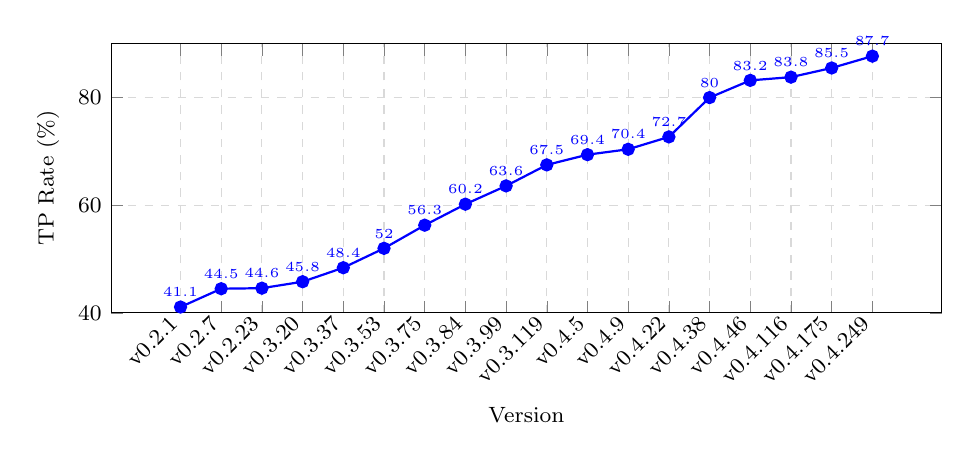
\begin{tikzpicture}
\begin{axis}[
    width=\columnwidth,
    height=5cm,
    xlabel={Version},
    ylabel={TP Rate (\%)},
    ymin=40, ymax=90,
    xtick=data,
    xticklabels={v0.2.1, v0.2.7, v0.2.23, v0.3.20, v0.3.37, v0.3.53, v0.3.75, v0.3.84, v0.3.99, v0.3.119, v0.4.5, v0.4.9, v0.4.22, v0.4.38, v0.4.46, v0.4.116, v0.4.175, v0.4.249},
    xticklabel style={rotate=45, anchor=east, font=\footnotesize},
    ylabel style={font=\footnotesize},
    xlabel style={font=\footnotesize},
    tick label style={font=\footnotesize},
    nodes near coords,
    nodes near coords style={font=\tiny},
    every node near coord/.append style={anchor=south},
    grid=major,
    grid style={dashed, gray!30},
]
\addplot[color=blue, mark=*, thick] coordinates {
    (1, 41.1) (2, 44.5) (3, 44.6) (4, 45.8) (5, 48.4) (6, 52.0) (7, 56.3) (8, 60.2) (9, 63.6) (10, 67.5) (11, 69.4) (12, 70.4) (13, 72.7) (14, 80.0) (15, 83.2) (16, 83.8) (17, 85.5) (18, 87.7)
};
\end{axis}
\end{tikzpicture}
\caption{TP rate progression from baseline (v0.2.1) through current
(v0.4.249).  The gap between v0.2.23 and v0.3.20 reflects the switch
from full-suite to fast-mode benchmarking.  The rate plateaus after
v0.4.46 despite continued FP-reduction work, reflecting the
diminishing-returns dynamic of \cref{sec:fp-reduction}.  The v0.4.175
point reflects a MEM30-C soundness fix that recovered CWE-416/415 TP
rate by 4--5 points each at zero added FP, but moves the aggregate
rate by only +0.1 points since both CWEs are a small share of the
79-CWE suite.  The plateau breaks at v0.4.249 (+2.2 points), driven by
a shared buffer-size-resolution consolidation across ARR30-C/ARR38-C/
STR31-C and a FIO30-C format-string fix (CWE-121/122/134 are the
largest movers); this is the largest single-version gain since
v0.4.46.  Between v0.4.116 and v0.4.175 (not separately plotted),
v0.4.139 enabled 15 previously-untracked rules, three of which
(MSC00-C, MSC11-C, MSC24-C) overlap existing Juliet CWEs; the
v0.4.175/v0.4.249 points are not purely FP-reduction movement (main
text).}
\label{fig:tp-rate-progression}
\end{figure}

\subsection{Competitor Comparison}
\label{sec:competitor}

\Cref{tab:competitor} compares SqC against four open-source tools on 15
overlapping Juliet CWEs.  All tools were run on the same test files with
TP/FP classified using identical Juliet ground truth (procedure names
and \texttt{OMITBAD}/\texttt{OMITGOOD} guards).

\begin{table*}[t]
\centering
\footnotesize
\setlength{\tabcolsep}{4pt}
\begin{tabular}{@{}llrrrrr@{}}
\toprule
\textbf{CWE} & \textbf{Description} & \textbf{SqC} & \textbf{cppcheck} & \textbf{clang-tidy} & \textbf{Infer} & \textbf{Frama-C} \\
\midrule
121 & Stack Buffer Overflow       & 74.8 & 40.5 & \textbf{86.6} & 38.8 & --- \\
122 & Heap Buffer Overflow        & 83.7 & 45.0 & \textbf{89.5} & 37.8 & --- \\
124 & Buffer Underwrite           & 70.9 & 40.5 & \textbf{90.4} & 33.9 & --- \\
127 & Buffer Underread            & 87.8 & 42.7 & \textbf{93.2} & 33.9 & --- \\
190 & Integer Overflow            & \textbf{100.0} & 27.5 & 94.3 & --- & 58.1 \\
191 & Integer Underflow           & \textbf{98.5} & 27.2 & 94.4 & --- & 63.1 \\
197 & Numeric Truncation          & \textbf{100.0} & 40.0 & 94.5 & --- & \textbf{100.0} \\
369 & Divide by Zero              & 61.4 & 27.4 & \textbf{94.7} & --- & 43.4 \\
401 & Memory Leak                 & 78.0 & 25.7 & \textbf{83.9} & 54.7 & --- \\
415 & Double Free                 & 62.8 & 33.8 & \textbf{80.0} & 63.0 & --- \\
416 & Use After Free              & \textbf{91.3} & 29.6 & 60.3 & 2.0  & --- \\
476 & Null Pointer Deref          & 67.9 & 39.7 & \textbf{94.3} & 66.1 & 64.2 \\
680 & Int Overflow $\to$ BOF      & \textbf{100.0} & 40.8 & 95.9 & --- & 82.6 \\
690 & Null Deref from Return      & \textbf{100.0} & 45.7 & 88.0 & 60.0 & --- \\
761 & Free Not at Start           & \textbf{100.0} & 45.7 & 94.3 & 58.1 & --- \\
\midrule
\multicolumn{2}{@{}l}{\textbf{Overall TP rate}} & 82.6 & 36.4 & \textbf{91.6} & 43.6 & 61.0 \\
\multicolumn{2}{@{}l}{\textbf{CWEs tested}}     & \textbf{79} & 15 & 15 & 10 & 6 \\
\bottomrule
\end{tabular}
\caption{TP rate (\%) comparison on overlapping Juliet CWEs.
\textbf{Bold} = highest per row.  ``---'' = CWE not tested by that tool.
SqC v0.4.271; cppcheck 2.10; clang-tidy (LLVM 21.1); Infer v1.2.0; Frama-C 32.0 EVA.
Competitor numbers are held fixed from the original study (not
re-measured); SqC's column reflects v0.4.271.
All tools run on same test files (28{,}488 total across 15 CWEs).}
\label{tab:competitor}
\end{table*}

Four patterns persist in this refreshed snapshot, which updates SqC's
column from v0.4.116 to v0.4.271 (155 releases, mostly real-world
FP-reduction work per \cref{sec:fp-reduction} rather than
Juliet-targeted tuning); the competitor columns are unchanged, held
fixed from the original study.  First, \textbf{clang-tidy still
achieves the highest overall precision} (91.6\%) with only 116 false
positives across all 15 CWEs, but the gap has continued to narrow:
SqC's overall rate on these 15 CWEs is now 82.6\% (up from 79.5\% at
v0.4.116, 68.2\% at the original snapshot), and it detects far more
total violations than clang-tidy (22{,}261 vs.\ 13{,}952 TP, though
note SqC's figure is summed over all 79 CWEs it tests, not just these
15).

Second, \textbf{SqC still beats clang-tidy outright on the same six
CWEs it won at v0.4.116}: CWE-190 (100.0\% vs.\ 94.3\%), CWE-191
(98.5\% vs.\ 94.4\%), CWE-416 (91.3\% vs.\ 60.3\%), CWE-680 (100.0\%
vs.\ 95.9\%), CWE-690 (100.0\% vs.\ 88.0\%), and CWE-761 (100.0\% vs.\
94.3\%), plus ties Frama-C at 100.0\% on CWE-197.  None of the 155
intervening releases flipped a row's winner in either direction; the
movement on the other nine rows is incremental (e.g.\ CWE-121 74.8\%
vs.\ 71.0\%, CWE-369 61.4\% vs.\ 57.8\%, CWE-415 62.8\% vs.\ 57.6\%)
rather than structural, consistent with the plateau-then-real-world-fix
pattern described in \cref{sec:fp-reduction} --- none of that work
targeted these 15 CWEs specifically.

Third, \textbf{SqC has further extended its lead over Frama-C}: 82.6\%
vs.\ Frama-C's 61.0\% on the 15 overlapping CWEs (was 79.5\% vs.\
61.0\% at v0.4.116, 68.2\% vs.\ 61.0\% at the original snapshot), while
covering 79 CWEs vs.\ Frama-C's 6.  SqC still exceeds Frama-C on
CWE-369 (61.4\% vs.\ 43.4\%), CWE-190 (100.0\% vs.\ 58.1\%), CWE-191
(98.5\% vs.\ 63.1\%), and CWE-680 (100.0\% vs.\ 82.6\%).

Fourth, \textbf{SqC wins on six CWEs outright}: CWE-190, CWE-680,
CWE-690, and CWE-761 at 100\%, CWE-191 at 98.5\%, and CWE-416
use-after-free (91.3\% vs.\ clang-tidy's 60.3\%), where MEM01-C's
flow-sensitive deref tracking after \texttt{free} distinguishes the
good/bad paths more reliably than clang-tidy's pattern checks.
CWE-416 has recovered slightly since v0.4.116 (90.7\%) and sits just
below the 92.9\% figure from the original study; it remains the clear
leader on this CWE regardless.

Fifth, \textbf{cppcheck still produces the most findings but the lowest
precision} (36.4\%), reflecting its heuristic approach.  Its 29{,}377
TPs represent high recall but at the cost of 51{,}361 FPs.

The coverage gap remains the key differentiator: SqC tests 79 CWEs
spanning 17 CERT~C categories, while the other tools cover 6--15 on
this benchmark.  A hypothetical ensemble of all five tools would
achieve both high per-CWE precision and broad coverage.

\subsection{Real-World Results}
\label{sec:realworld-results}

\Cref{tab:realworld-results} compares SqC against cppcheck and
clang-tidy across the 9-project real-world set. seL4 has no
cppcheck/clang-tidy baseline yet (onboarded as a ninth oracle after the
last competitor sweep); sqlite's scan scope narrowed between versions
(125$\to$81 in-scope files) as its file predicate was tightened, not a
regression.

\begin{table}[t]
\centering
\footnotesize
\begin{tabular}{@{}lrrr@{}}
\toprule
\textbf{Project} & \textbf{sqc} & \textbf{cppcheck} & \textbf{clang-tidy} \\
\midrule
libcrc & 395 & 40 & 2 \\
lua & 3,047 & 49 & 107 \\
raylib & 4,749 & 1,060 & 469 \\
mosquitto & 2,970 & 277 & 44 \\
curl & 8,582 & 556 & 116 \\
sqlite & 18,922 & 503 & 137 \\
hostap & 30,752 & 1,761 & 1,710 \\
pure-ftpd & 5,855 & 12 & 109 \\
seL4 & 4,959 & --- & --- \\
\midrule
\textbf{Total} & \textbf{80,231} & \textbf{4,258} & \textbf{2,694} \\
\bottomrule
\end{tabular}
\caption{Violation counts (sqc v0.4.249, cppcheck v2.10, clang-tidy
v21.1.6).  Excluding seL4 (no competitor baseline), SqC's total is
75,272 across the other 8 projects --- an $\sim$18--28$\times$
difference vs.\ cppcheck/clang-tidy, reflecting SqC's 311-rule coverage
vs.\ $\sim$20 checks in competitors.  SqC's own total dropped 28\% from
the v0.4.120 figure (104,733 across the original 7 projects) despite
covering more rules, from the FP-reduction work in
\cref{sec:fp-reduction} landing on real-world code, not just Juliet.}
\label{tab:realworld-results}
\end{table}

Beyond raw violation volume, what matters is what fraction of these
findings are real: scored against a hand-adjudicated ground-truth
oracle spanning all 9 projects (\cref{sec:ground-truth-snapshot}), aggregate
measured precision is 16.6\% (TP 10,561 of 63,608 labeled findings) with
97.4\% recall (10,561 of 10,841 known true positives flagged), at 86.3\%
label coverage (63,649 of 73,718 total findings labeled;
run \texttt{sqc-0.4.258}). As with the Juliet 100\%-precision figures
in \cref{tab:perfect-cwes}, this aggregate number should be read scoped
to its oracle rather than as a universal precision claim
(\cref{sec:limitations}).

\Cref{tab:realworld-timing} reports analysis throughput.  Each tool was
run serially---one process at a time, with the full machine to itself---so
the durations are uncontended wall-clock process runtime; throughput is
LOC divided by that runtime.  LOC is physical lines over the same curated
source scope used as the denominator for all three tools.

\begin{table}[t]
\centering
\footnotesize
\setlength{\tabcolsep}{4pt}
\resizebox{\columnwidth}{!}{%
\begin{tabular}{@{}lrrrr@{}}
\toprule
& & \multicolumn{3}{c}{\textbf{Time (s) / Throughput (LOC\,s$^{-1}$)}} \\
\cmidrule(l){3-5}
\textbf{Project} & \textbf{LOC} & \textbf{sqc} & \textbf{cppcheck} & \textbf{clang-tidy} \\
\midrule
libcrc & 1,034 & 0.6 / 1,723 & 0.1 / 10,340 & 0.1 / 10,340 \\
mosquitto & 39,368 & 22.6 / 1,741 & 3,278.8 / 12 & 2.3 / 17,116 \\
curl & 186,220 & 72.5 / 2,568 & 642.5 / 289 & 4.8 / 38,795 \\
sqlite & 218,733 & 165.5 / 1,321 & 1,198.7 / 182 & 7.0 / 31,247 \\
hostap & 589,724 & 353.1 / 1,670 & 2,659.3 / 221 & 55.9 / 10,549 \\
\bottomrule
\end{tabular}}
\caption{Real-world analysis time and throughput (sqc v0.4.55,
cppcheck v2.10, clang-tidy v21.1.6), measured serially to avoid CPU
contention.  SqC throughput is stable at $\sim$1{,}300--2{,}600\,LOC\,s$^{-1}$
across codebases.  cppcheck is intrinsically slow---54.6\,min on
mosquitto (12\,LOC\,s$^{-1}$) despite its small size---rather than
contention-bound.  clang-tidy is fastest here but runs a narrower check
set (cf.~its violation counts in \cref{tab:realworld-results}), so its
throughput is not directly comparable on analysis depth.  This table has
not been re-measured since v0.4.55: the automated benchmark harness now
runs projects concurrently for throughput, so its per-run duration
figures (\cref{sec:realworld-results}) are not directly comparable to
the strict single-process, uncontended protocol this table requires.
A fresh controlled re-measurement at the current version is future work;
the per-CWE scan-time trend below (\cref{fig:scan-time}), which is
contention-independent by construction, is the up-to-date proxy for
how analysis cost has evolved since v0.4.55.}
\label{tab:realworld-timing}
\end{table}

\Cref{fig:realworld-reduction} shows that FP reductions developed on
Juliet transfer to real-world code in the aggregate: total violations
across the original five codebases dropped 82.4\% from v0.2.7 to
v0.4.120, though nearly all of that reduction had already landed by
v0.4.22 --- the subsequent 98 releases removed a further 27.7\% on top
of the v0.4.22 figure, another instance of the diminishing-returns
pattern (\cref{fig:tp-rate-progression}).
(\Cref{sec:limitations} shows the important caveat: aggregate volume
reduction does not imply real-world precision.)

\begin{figure}[t]
\centering
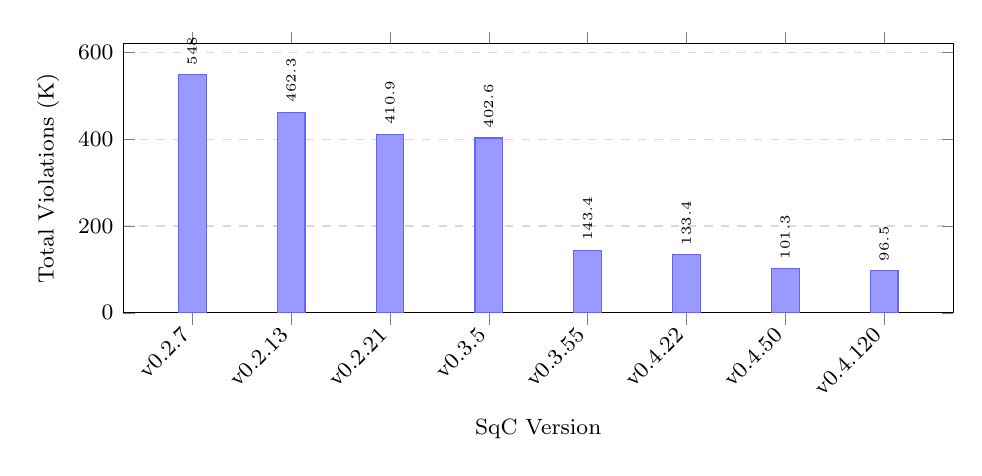
\begin{tikzpicture}
\begin{axis}[
    width=\columnwidth,
    height=5cm,
    ybar,
    xlabel={SqC Version},
    ylabel={Total Violations (K)},
    ymin=0, ymax=620,
    xtick=data,
    xticklabels={v0.2.7, v0.2.13, v0.2.21, v0.3.5, v0.3.55, v0.4.22, v0.4.50, v0.4.120},
    xticklabel style={rotate=45, anchor=east, font=\footnotesize},
    ylabel style={font=\footnotesize},
    xlabel style={font=\footnotesize},
    tick label style={font=\footnotesize},
    bar width=10pt,
    nodes near coords,
    nodes near coords style={font=\tiny, rotate=90, anchor=west},
    ymajorgrids=true,
    grid style={dashed, gray!30},
]
\addplot[fill=blue!40, draw=blue!60] coordinates {
    (1, 548.0)
    (2, 462.3)
    (3, 410.9)
    (4, 402.6)
    (5, 143.4)
    (6, 133.4)
    (7, 101.3)
    (8, 96.5)
};
\end{axis}
\end{tikzpicture}
\caption{Total SqC violations across the original 5 real-world
codebases by version (libcrc, mosquitto, curl, sqlite, hostap; lua and
raylib excluded here for continuity with the pre-v0.4.83 series).
Reduction v0.2.7$\to$v0.4.120: $-$451,506 ($-$82.4\%).}
\label{fig:realworld-reduction}
\end{figure}

For the one rule where all three tools have overlapping coverage
(null pointer dereference), the difference in analysis philosophy is
stark.  On mosquitto, SqC reports 386 EXP34-C violations at v0.4.120
(down from 8,657 at v0.3.5, and further down from 504 at v0.4.22)
compared to cppcheck's 2 \texttt{nullPointer} findings.  cppcheck fires
only when it can \emph{prove} a null dereference path exists; SqC flags
all paths that \emph{may} dereference a null pointer.  This is a
fundamental tradeoff between coverage and precision that different
users will weight differently, and the adjudicated oracle
(\cref{sec:limitations}) quantifies its cost: even after a
22$\times$ volume reduction, EXP34-C's measured precision across the
six audited projects (curl, hostap, lua, mosquitto, raylib, sqlite) is
0.66\% (15 TP / 2{,}264 labeled), so the overwhelming majority of
EXP34-C findings on real-world code are still false positives ---
starkly at odds with CWE-690's 100\% precision on Juliet
(\cref{tab:perfect-cwes}); EXP34-C also covers CWE-476, so its own
Juliet-wide FP rate is a more modest 13\% (\cref{tab:top-rules}), but
even that headline number does not survive contact with real-world
code.

That low precision coexists with a concentrated pocket of confirmed
true positives.  Delta-adjudicating EXP34-C's findings against
SQLite's \texttt{ext/} extension modules --- code reachable only
through optional loadable extensions, and correspondingly less
scrutinized than the core engine --- confirmed 11 genuine
out-of-memory-triggered NULL-dereference bugs: an unchecked
\texttt{sqlite3\_malloc64()} result used directly in \texttt{fread()}
(\texttt{ext/expert/expert.c}); \texttt{sqlite3\_column\_name()}
strlen'd with no NULL check at two sites in
\texttt{ext/fts3/fts3.c}; \texttt{sqlite3\_column\_text()} indexed and
compared with no NULL check in \texttt{ext/misc/amatch.c} (SQL-NULL
triggerable, not merely OOM); \texttt{sqlite3\_vmprintf()} consumed
unguarded at two sites in \texttt{ext/misc/sqlite3\_stdio.c};
\texttt{sqlite3\_stmt\_scanstatus\_v2()}'s
\texttt{SQLITE\_SCANSTAT\_EXPLAIN} output used unguarded on its normal
(non-error) return path in \texttt{ext/qrf/qrf.c}; and an
\texttt{sqlite3\_mprintf()} result passed to plain libc \texttt{printf}'s
\texttt{\%s} --- bypassing SQLite's own NULL-safe \texttt{mprintf} ---
in \texttt{ext/session/changeset.c}.  Cross-checking against the live
upstream mainline found 4 of the original 11 sites already
independently hardened by a June 2026 OOM-hardening pass; we filed
disclosures for the remaining six, covering
\texttt{expert.c}\footnote{\url{https://sqlite.org/bugs/forumpost/c06a3c0d3f}},
\texttt{amatch.c}\footnote{\url{https://sqlite.org/bugs/forumpost/20d89d613b}},
\texttt{sqlite3\_stdio.c}\footnote{\url{https://sqlite.org/bugs/forumpost/ba00fdddda}},
\texttt{changeset.c}\footnote{\url{https://sqlite.org/bugs/forumpost/f20ea456ac}},
\texttt{fts3.c}\footnote{\url{https://sqlite.org/bugs/forumpost/9b4276628a}},
and \texttt{qrf.c}\footnote{\url{https://sqlite.org/bugs/forumpost/18338dc19d}}.
SQLite fixed all six the same day they were filed, extending the
same-day/next-day turnaround documented in
\cref{sec:provenance-frontier} to nine consecutive disclosures across
this evaluation.  Unlike the \texttt{kvvfsDecode} finding in
\cref{sec:provenance-frontier} (an audit-discovered false negative,
not a rule detection), these 11 sites are genuine EXP34-C true
positives --- the rule flagged real bugs, adjudication confirmed them
against source, and the resulting disclosures were externally
validated by the same-day fixes.  They are a small fraction of
EXP34-C's real-world output, but a concrete demonstration that its
0.66\% measured precision reflects volume of false alarms, not an
absence of genuine findings underneath them.

\subsection{A Defect Class Juliet Cannot Surface}
\label{sec:juliet-blindspot}

The precision gap above is the expected direction of disagreement:
Juliet flatters a rule that misbehaves in the field.  The real-world
oracles also disagree in the \emph{opposite} direction---they expose
defects in the analyzer that Juliet structurally cannot report at all.
The clearest case is a class of duplicate-finding bugs, where a rule
emits the same diagnostic more than once for a single program fact.

A complete adjudication of our fifth oracle, Lua~5.5
(\texttt{lgc.c}~@\,\texttt{40b76de2}), surfaced the severe form.  DCL02-C
(visually similar identifiers) re-emitted the identical \texttt{n}/\texttt{h}
diagnostic 100~times on each of two source lines: 200 of the rule's
203 findings on that file were exact duplicates of just two real
diagnostics (\cref{tab:dup-class}).  The root cause was an
$O(\text{depth})$ re-traversal---the rule re-analyzed each enclosing
block, re-emitting once per pairwise comparison rather than once per
declaration site---so the duplication factor scales with block-nesting
depth.  Juliet never surfaced this: its synthetic test cases are small
and shallow, and none reaches the nesting depth at which the blow-up
becomes visible.

Prompted by that finding, we audited the same bug \emph{class} across
the rule set and found milder, constant-factor instances whose inputs
\emph{were} present in Juliet: POS37-C emitted every dropped-privilege
finding twice (2.0$\times$, all CWE273 cases), SIG31-C emitted some
shared-object accesses twice (1.5$\times$, CWE364), and FIO42-C reported
one resource under two mutually exclusive messages---unclosed
\texttt{FILE*} \emph{and} unclosed file descriptor---a misclassification
inflating CWE404 by 1.53$\times$.  Crucially, Juliet's pass/fail oracle
could not flag even these: a Juliet \texttt{bad} case passes when the
finding set for the seeded defect is non-empty, so a duplicated or
misclassified finding scores identically to a single correct one.  The
metric is count-blind by construction; the defects were latent in the
Juliet corpus but invisible to its scoring.

\begin{table}[t]
\centering
\footnotesize
\setlength{\tabcolsep}{4pt}
\begin{tabular}{@{}llrl@{}}
\toprule
\textbf{Rule} & \textbf{Surfaced by} & \textbf{Factor} & \textbf{Mechanism} \\
\midrule
DCL02-C & Lua (real-world)  & 100$\times$  & $O(\text{depth})$ re-traversal \\
POS37-C & Juliet CWE273     & 2.0$\times$  & subtree visited twice \\
SIG31-C & Juliet CWE364     & 1.5$\times$  & per-reference emit \\
FIO42-C & Juliet CWE404     & 1.53$\times$ & opener misclassification \\
\bottomrule
\end{tabular}
\caption{Duplicate-finding defects.  DCL02-C's scale-dependent form
(200 of 203 \texttt{lgc.c} findings were duplicates of two lines) was
reachable only through real-world depth; the constant-factor forms were
present in Juliet inputs but invisible to its presence-based oracle.
All four are fixed at the rule level (v0.4.58--v0.4.63).}
\label{tab:dup-class}
\end{table}

These are two distinct blind spots, and the real-world oracle covers
both.  The first is one of \emph{scale}: synthetic micro-benchmarks do
not exercise the depth, size, and idiom at which structural or
algorithmic defects manifest.  The second is one of \emph{oracle
granularity}: a presence-based pass/fail metric cannot detect
over-emission at any scale, whereas the real-world audit counts and
inspects every individual finding.  This is direct evidence that the
six real-world oracles complement Juliet rather than duplicate it:
they measure deployment precision (\cref{sec:limitations}), and they
exercise the analyzer at a scale and granularity Juliet does not reach.

\subsection{Runtime Performance}
\label{sec:runtime}

To characterize SqC's runtime behavior across hardware configurations,
we ran single-process scans (cross-file analysis enabled, no prescan
cache) on four machines (\cref{tab:testbed}).

\begin{table}[t]
\centering
\footnotesize
\begin{tabular}{@{}clccc@{}}
\toprule
\textbf{ID} & \textbf{CPU} & \textbf{Cores} & \textbf{RAM} & \textbf{Disk} \\
\midrule
M1 & Xeon E5-2640 @ 2.50\,GHz & 6/24 & 192\,GB & SSD \\
M2 & Ryzen 5 PRO 2400GE @ 3.20\,GHz & 4/8  & 16\,GB  & SSD \\
M3 & i7-7700T @ 2.90\,GHz    & 4/8  & 16\,GB  & SSD \\
M4 & i7-9750H @ 2.60\,GHz    & 6/12 & 16\,GB  & HDD \\
\bottomrule
\end{tabular}
\caption{Test machines.  Cores listed as physical/logical.
All run Linux 6.x.  M1 is a rack server; M2--M4 are desktop/laptop
class.}
\label{tab:testbed}
\end{table}

\Cref{tab:runtime} shows wall-clock times for single-process analysis
of sqlite (404K LOC) across all four machines with cross-file analysis
enabled and no prescan cache (cold start).

\begin{table}[t]
\centering
\footnotesize
\begin{tabular}{@{}crr@{}}
\toprule
\textbf{Machine} & \textbf{Time (s)} & \textbf{LOC/s} \\
\midrule
M1 & 3{,}470 & 117 \\
M2 & 3{,}116 & 130 \\
M3 & 2{,}363 & 171 \\
M4 & 1{,}986 & 204 \\
\bottomrule
\end{tabular}
\caption{Single-process analysis time for sqlite (404,701 LOC,
cross-file analysis enabled, cold cache).}
\label{tab:runtime}
\end{table}

\textbf{Scaling across codebases.}
\Cref{tab:runtime-scaling} shows how throughput varies with codebase
size on M1.  Throughput generally decreases for larger codebases
because cross-file analysis cost grows with the number of
inter-procedural edges.  The exception is sqlite, whose throughput
(117 LOC/s) is lower than the larger hostap (155 LOC/s).  This is
because sqlite ships as a single 230K-line amalgamation file
(\texttt{sqlite3.c}) with dense internal cross-references, whereas
hostap distributes its code across 504 files averaging $\sim$1{,}070
LOC each.  Per-file analysis cost is dominated by intra-file
complexity, not total codebase size.

\begin{table}[t]
\centering
\footnotesize
\begin{tabular}{@{}lrrr@{}}
\toprule
\textbf{Project} & \textbf{LOC} & \textbf{Time (s)} & \textbf{LOC/s} \\
\midrule
libcrc    &   2{,}130 &     2 &   888 \\
mosquitto &  88{,}717 &   172 &   516 \\
curl      & 240{,}331 &   609 &   395 \\
hostap    & 539{,}617 & 3{,}479 & 155 \\
sqlite    & 404{,}701 & 3{,}470 & 117 \\
\bottomrule
\end{tabular}
\caption{Single-process throughput on M1 across all five benchmark
codebases (cross-file analysis, cold cache).  sqlite's lower
throughput despite fewer LOC than hostap reflects the cost of
analyzing its 230K-line amalgamation file.}
\label{tab:runtime-scaling}
\end{table}

In single-process mode, loading a cached prescan saves less than 1\%
of wall time---the prescan is a small fraction of total analysis cost.
The cache's primary benefit is enabling parallel analysis.

\textbf{Parallel mode.}  SqC provides built-in file-level parallelism
via the \texttt{-j}/\texttt{-{}-jobs} flag (default: auto-detect CPU
count).  Each worker thread receives its own parser and rule registry
instance, avoiding shared mutable state.  After a single-threaded
prescan builds the cross-file context (function summaries, call graph,
null states), files are analyzed in parallel with results merged
deterministically.

\textbf{LPT scheduling.}  Real-world C codebases exhibit highly skewed
file-size distributions: curl's largest file (169\,KB) is 44$\times$
the median, and sqlite's amalgamation file (630\,KB) is 37$\times$ the
median.  Na\"ive parallel dispatch can leave threads idle while a
straggler processes a large file.  SqC applies Graham's
Longest-Processing-Time-first (LPT) heuristic~\cite{graham-lpt}: files
are sorted by size in descending order and dispatched via demand-driven
scheduling, where each thread pulls the next unprocessed file upon
becoming idle.  This achieves a $(4/3 - 1/3m)$-approximation to the
optimal makespan, where $m$ is the thread count.

\Cref{tab:parallel} shows the impact on a 24-core server.  LPT
scheduling reduces worst-case latency by 6--9\% and, critically,
reduces run-to-run variance by 52--99\%, making analysis times
predictable for CI/CD integration.

\begin{table}[t]
\centering
\footnotesize
\begin{tabular}{@{}llrrrr@{}}
\toprule
\textbf{Project} & \textbf{Mode} & \textbf{Avg (s)} & \textbf{Worst (s)} & \textbf{$\sigma$ (s)} & \textbf{CPU eff.} \\
\midrule
curl    & par\_iter (baseline) & 178.5 & 193.4 & 13.0 & --- \\
curl    & LPT + par\_bridge   & 176.4 & 176.5 &  0.1 & --- \\
\addlinespace
sqlite  & par\_iter (baseline) & 1{,}197 & 1{,}280 & 71.8 & 83\% \\
sqlite  & LPT + par\_bridge   & 1{,}169 & 1{,}204 & 34.3 & 96\% \\
\bottomrule
\end{tabular}
\caption{LPT scheduling impact at $-j\,4$ (3 runs each, cross-file
analysis enabled).  CPU efficiency is CPU time divided by wall time
divided by thread count; 100\% means zero idle time.  LPT's primary
benefit is variance reduction and worst-case improvement, not average
speedup.}
\label{tab:parallel}
\end{table}

The Juliet benchmark (70 CWEs, fast mode) completes in approximately
15 minutes on the 24-core server using per-CWE parallelism.

\textbf{Scan time across versions.}  Because per-CWE timing is recorded
for every benchmark run, we can track how analysis cost evolved as rules
and inter-procedural depth were added.  \Cref{fig:scan-time} plots scan
time per CWE---the summed per-CWE \texttt{sqc} analysis time divided by
the number of CWEs scanned---across 108 released versions.  This metric
is independent of both the parallelism setting (\texttt{-{}-jobs}) and
corpus growth (the matched CWE set expanded from 68 to 74 over the
window), making it comparable across the full history.  Two features
stand out.  A single optimization at v0.3.67 cut per-CWE time roughly
8$\times$ (from $\approx$230\,s to $\approx$27\,s).  The subsequent climb
back to $\approx$130\,s is the price of the cross-file prescan and
dataflow analysis introduced over the v0.3.9x--v0.4.x series; notably,
even with this added depth the tool settles well below its earlier
v0.3.5x peak of $\approx$298\,s per CWE.

% Auto-generated by scripts/benchmark_timing_figure.py -- do not edit by hand.
% Juliet scan time per CWE (parallelism- and corpus-size-independent), v0.3.25-v0.4.45.
\begin{figure}[t]
\centering
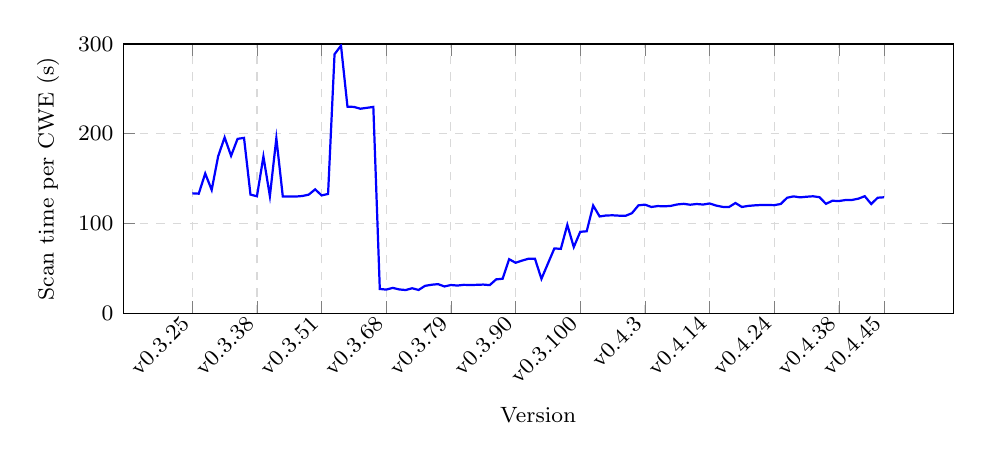
\begin{tikzpicture}
\begin{axis}[
    width=\columnwidth,
    height=5cm,
    xlabel={Version},
    ylabel={Scan time per CWE (s)},
    ymin=0, ymax=300,
    xtick={1, 11, 21, 31, 41, 51, 61, 71, 81, 91, 101, 108},
    xticklabels={v0.3.25, v0.3.38, v0.3.51, v0.3.68, v0.3.79, v0.3.90, v0.3.100, v0.4.3, v0.4.14, v0.4.24, v0.4.38, v0.4.45},
    xticklabel style={rotate=45, anchor=east, font=\footnotesize},
    ylabel style={font=\footnotesize},
    xlabel style={font=\footnotesize},
    tick label style={font=\footnotesize},
    grid=major,
    grid style={dashed, gray!30},
]
\addplot[color=blue, thick, mark=none] coordinates {
    (1, 133.6) (2, 133.2) (3, 155.7) (4, 137.4) (5, 174.9) (6, 195.9) (7, 175.4) (8, 194.3) (9, 195.4) (10, 132.2) (11, 130.3) (12, 174.6) (13, 130.5) (14, 195.0) (15, 130.0) (16, 130.0) (17, 130.0) (18, 130.6) (19, 132.1) (20, 138.0) (21, 131.3) (22, 132.9) (23, 288.6) (24, 298.2) (25, 230.2) (26, 229.9) (27, 227.9) (28, 228.9) (29, 229.9) (30, 27.0) (31, 26.3) (32, 28.2) (33, 26.5) (34, 25.8) (35, 27.8) (36, 25.9) (37, 30.5) (38, 31.7) (39, 32.4) (40, 29.8) (41, 31.4) (42, 30.8) (43, 31.6) (44, 31.4) (45, 31.6) (46, 31.9) (47, 31.3) (48, 37.7) (49, 38.4) (50, 60.2) (51, 56.2) (52, 58.6) (53, 60.7) (54, 60.6) (55, 38.3) (56, 55.3) (57, 72.2) (58, 71.7) (59, 98.5) (60, 73.7) (61, 90.7) (62, 91.3) (63, 120.0) (64, 107.8) (65, 108.9) (66, 109.1) (67, 108.7) (68, 108.5) (69, 111.5) (70, 120.2) (71, 121.0) (72, 118.4) (73, 119.4) (74, 119.1) (75, 119.6) (76, 121.2) (77, 121.9) (78, 120.9) (79, 121.7) (80, 121.1) (81, 122.3) (82, 120.0) (83, 118.5) (84, 118.3) (85, 122.8) (86, 118.4) (87, 119.6) (88, 120.2) (89, 120.6) (90, 120.6) (91, 120.4) (92, 121.7) (93, 128.7) (94, 130.2) (95, 129.1) (96, 129.8) (97, 130.3) (98, 129.3) (99, 121.9) (100, 125.3) (101, 125.0) (102, 126.1) (103, 126.2) (104, 127.6) (105, 130.4) (106, 121.7) (107, 128.7) (108, 129.2)
};
\end{axis}
\end{tikzpicture}
\caption{Juliet scan time per CWE across 108 released versions
(v0.3.25--v0.4.45). The metric is the summed
per-CWE \texttt{sqc} analysis time divided by the number of CWEs scanned,
making it independent of both parallelism (\texttt{--jobs}) and corpus growth
(68--74 CWEs). The sharp drop at v0.3.67 is a single perf optimization
($\approx$8$\times$); the subsequent climb is the cost of added
inter-procedural analysis, which still settles below the v0.3.5x peak.}
\label{fig:scan-time}
\end{figure}



%% ============================================================
\section{Iterative False Positive Reduction}
\label{sec:fp-reduction}

Reducing false positives while maintaining detection is the central
engineering challenge for a broad-coverage static analyzer.  This
section walks through the techniques that improved the TP rate from
41.1\% to 83.8\%, organized by the insight that motivated each change.

\Cref{fig:fp-reduction} shows the TP and FP counts across 12
optimization rounds.

\begin{figure}[t]
\centering
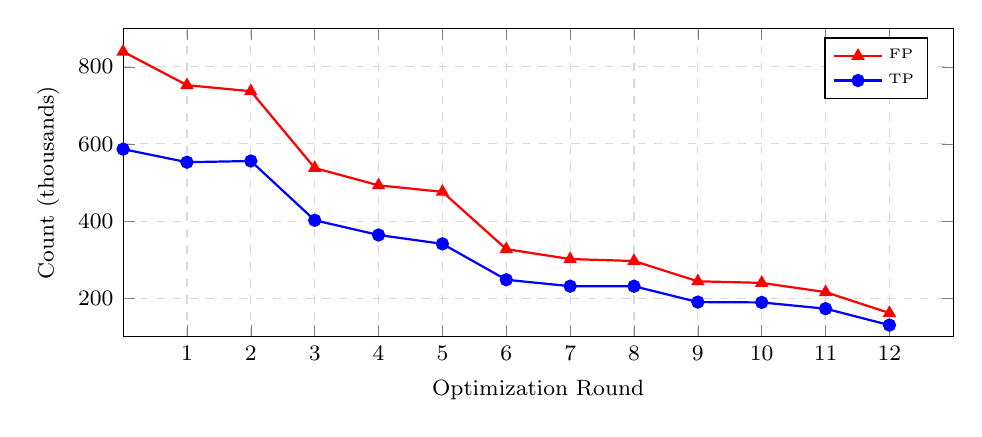
\begin{tikzpicture}
\begin{axis}[
    width=\columnwidth,
    height=5.5cm,
    xlabel={Optimization Round},
    ylabel={Count (thousands)},
    ymin=100, ymax=900,
    xmin=0, xmax=13,
    xtick={1,2,3,4,5,6,7,8,9,10,11,12},
    ylabel style={font=\footnotesize},
    xlabel style={font=\footnotesize},
    tick label style={font=\footnotesize},
    grid=major,
    grid style={dashed, gray!30},
    legend style={font=\tiny, at={(0.97,0.97)}, anchor=north east},
]
\addplot[color=red, mark=triangle*, thick] coordinates {
    (0, 839.3)
    (1, 752.4) (2, 736.6) (3, 537.6) (4, 492.6)
    (5, 475.8) (6, 327.2) (7, 301.5) (8, 296.4)
    (9, 243.8) (10, 239.7) (11, 215.7) (12, 161.5)
};
\addlegendentry{FP}
\addplot[color=blue, mark=*, thick] coordinates {
    (0, 586.5)
    (1, 552.6) (2, 555.7) (3, 402.0) (4, 363.9)
    (5, 340.9) (6, 247.8) (7, 231.1) (8, 231.0)
    (9, 189.9) (10, 189.0) (11, 172.8) (12, 130.2)
};
\addlegendentry{TP}
\end{axis}
\end{tikzpicture}
\caption{TP and FP counts across optimization rounds (full Juliet
suite, thousands).  Both decline as overly-broad rules are tightened;
the key metric is TP rate, which improved from 41.1\% to 44.6\%.}
\label{fig:fp-reduction}
\end{figure}

\subsection{The Header Problem}
\label{sec:fp-cross-file}

The first and largest source of false positives came from a fundamental
limitation of the tree-sitter approach: without \texttt{\#include}
resolution, every call to a function defined in another file looks like
a call to an undeclared function.  Rules DCL31-C and DCL07-C would flag
every \texttt{malloc()}, \texttt{printf()}, and \texttt{CreateFile()}
call.

The fix came in two stages.  First, a built-in database of standard
functions (Round 3, $-$198,974 FPs).  Second, cross-file analysis: a
pre-scan of project directories to discover all function definitions
(Round 6, $-$148,622 FPs).  Together, these two changes account for
41\% of the total FP reduction.

Later, adding $\sim$100 Windows API functions to the database
(Round 9) removed another 36K FPs from DCL31-C/DCL07-C alone---the
biggest single-rule win of any round.

\subsection{Type-Aware Analysis}

Several integer rules initially operated on the text of expressions
without considering the types of the operands.  This produced false
positives on non-integer types:

\begin{itemize}
    \item \texttt{char data; data + 1} was flagged as signed integer
        overflow (INT32-C).  Fix: \texttt{infer\_type()} returns
        ``not applicable'' for non-integer types.
    \item \texttt{ptr + n} was flagged as unsigned integer wrap
        (INT30-C).  Fix: pointer arithmetic is identified as valid C.
    \item Float-to-int assignments with unknown types were flagged
        (FLP34-C).  Fix: only flag when both sides have known,
        mismatched types.
\end{itemize}

The lesson: \emph{don't flag when uncertain.}  Suppressing warnings
for unknown or ambiguous types consistently improved the FP-to-TP
ratio.

\subsection{Bounds-Check Detection}

INT32-C and INT30-C gained AST-ancestor walking to detect enclosing
bounds checks.  The algorithm walks up to 15 ancestors looking for an
enclosing \texttt{if\_statement} whose condition references a type-limit
macro (\texttt{INT\_MAX}, \texttt{UINT64\_MAX}, etc.) \emph{and} at
least one arithmetic operand.

This achieved a 12.5:1 FP-to-TP reduction ratio for INT32-C.  One
important implementation detail: we use word-boundary matching for
macro names, because \texttt{ULONG\_MAX} contains \texttt{LONG\_MAX}
as a substring.

\subsection{Constant Evaluation}

The constant evaluator resolves $\sim$35 C standard limit macros,
$\sim$20 type sizes via \texttt{sizeof}, and arithmetic on these
values.  This produced the largest single-round FP reduction since
cross-file analysis ($-$12,088 FPs in Round 12), because it enabled
every integer rule to reason about allocation sizes, buffer bounds,
and guard conditions.

\subsection{Diminishing Returns}

\Cref{tab:fp-milestones} shows selected milestones.  The pattern of
diminishing returns is clear: Round 3 removed 199K FPs; by Round 8,
only 5K.  Each successive round requires more sophisticated analysis
for smaller gains.

\begin{table}[t]
\centering
\footnotesize
\begin{tabular}{@{}rlrrr@{}}
\toprule
\textbf{Rd} & \textbf{Key Change} & \textbf{FP} & \textbf{$\Delta$FP} & \textbf{TP\%} \\
\midrule
0 & Baseline (full suite) & 839K & --- & 41.1 \\
3 & Std function DB & 538K & $-$199K & 42.8 \\
6 & Cross-file analysis & 327K & $-$149K & 43.1 \\
9 & Windows API + types & 244K & $-$53K & 43.8 \\
12 & Const eval + macros & 162K & $-$12K & 44.6 \\
\midrule
\multicolumn{5}{@{}l}{\emph{Switch to fast-mode benchmarking (v0.3.20)}} \\
\midrule
--- & Fast-mode baseline & 24.7K & --- & 45.8 \\
--- & VRA + buffer analysis & 18.8K & $-$5.9K & 56.3 \\
--- & CFG const + CWE-369 & 17.0K & $-$1.8K & 60.2 \\
--- & Taint + return-value   & 14.1K & $-$2.9K & 63.6 \\
v0.3.119 & Precision improvements & 11.7K & $-$2.4K & 67.5 \\
v0.4.22 & VRA + STR31-C + EXP33-C & 9.9K & $-$1.8K & 72.7 \\
v0.4.46 & Opt-in INT provenance gating & 4.6K & $-$5.3K & 83.2 \\
v0.4.116 & Per-rule tuning (plateau) & 4.2K & $-$0.4K & 83.8 \\
\bottomrule
\end{tabular}
\caption{FP reduction milestones.  Full-suite rounds 0--12 reduced FP by
80.7\%.  Fast-mode continued from 45.8\% to 83.8\% TP rate.  The v0.4.22
row reflects continued VRA improvements, STR31-C buffer-size inference,
EXP33-C inter-procedural FP suppression, and crash-robustness fixes that
unlocked previously-aborted scans (raising both TP and FP).  v0.4.46
reflects the opt-in provenance-gated rewrite of INT30/31/32-C
(\cref{sec:provenance-frontier}), the single largest FP reduction since
cross-file analysis.  The 70 releases from v0.4.46 to v0.4.116 removed
only a further 0.4K FP (0.2 points of TP rate), the diminishing-returns
pattern continuing to its current extreme.}
\label{tab:fp-milestones}
\end{table}

\subsection{Principles That Emerged}

Five principles emerged from this iterative process:

\begin{enumerate}
    \item \textbf{Don't flag when uncertain.}  If the type, origin,
        or value of an operand is unknown, suppress the warning.
    \item \textbf{Target absolute FP counts, not rates.}  A rule with
        99\% FP rate and 100 violations matters less than one with
        50\% FP rate and 10K violations.
    \item \textbf{Zero-TP rules are free FP reductions.}  DCL40-C's
        31-character identifier prefix check produced 12K FPs and 0 TPs
        on Juliet.  Removing it was cost-free.
    \item \textbf{Verify on both benchmarks.}  Fixes targeting
        \texttt{uint32\_t} resolution show impact on real-world code
        but not on Juliet, which uses explicit C types.
    \item \textbf{Juliet is a rough approximation, not a proxy.}
        Treat the real-world suite as a first-class benchmark, run
        with the same rigor (versioned, committed, per-rule deltas
        reviewed) as Juliet.  Real-world code crashed the analyzer in
        ways Juliet structurally cannot (non-ASCII content,
        thousands-deep nesting, adversarial token ordering), exhibited
        per-rule regressions that Juliet scored as neutral or
        improved, and a sampled manual audit of the noisiest rules
        measured real-world precision far below what Juliet results
        implied.  Improvements validated only on Juliet have not, in
        our experience, earned the claim of working on real code.
\end{enumerate}

\subsection{The Residual Frontier: Provenance over Proof}
\label{sec:provenance-frontier}

The five principles above are all \emph{opt-out} refinements: each
suppresses a warning that sqc cannot prove dangerous.  A complete
file-at-a-time audit of SQLite---220 files at commit
\texttt{b1a73ba34d}, with every finding manually adjudicated---shows
where this philosophy reaches its limit.  INT32-C (signed integer
overflow) emitted 4{,}420 false positives against 15 true positives
(0.3\% precision), alone accounting for roughly one fifth of all of
sqc's false positives on the project.  Tracing the flagged source
lines is clarifying.  Every false positive is plain arithmetic on a
\emph{bounded} local integer---a register index (\texttt{regData-1}),
a statement counter (\texttt{db->nStatement-{}-}), a small loop count
(\texttt{nIdx+1}), a page-size sum (\texttt{szPage+szExtra}).  All 15
true positives involve an operand derived from \emph{untrusted,
unbounded} input: a varint decoded from a database blob, an
attacker-controlled cell count, a length read from a file, a value
parsed from the command line.  The discriminator is not the operation
but the \emph{provenance} of its operands.

This is not a value-range tuning problem.  sqc's VRA already proves
safety wherever a bound is visible; the residual false positives are
exactly the cases where the bound is a program invariant the analyzer
cannot see---a \texttt{SQLITE\_LIMIT} constant, an \texttt{assert}, a
data-structure size.  The bounded \texttt{nIdx+1} and the genuinely
dangerous \texttt{data+1} (where \texttt{data} came from
\texttt{atoi}) are \emph{syntactically identical}; only the origin of
the variable distinguishes them, so no amount of local proof closes
the gap.

The static-analysis literature splits cleanly on how to resolve this
(\cref{tab:optout-optin}).  Sound abstract-interpretation tools---%
Frama-C's Eva plugin~\cite{frama-c}, Infer's Inferbo buffer-overrun
domain~\cite{inferbo}, and CodeQL's range-analysis
library~\cite{codeql-range}---are \emph{opt-out}: they compute an
over-approximated (often \emph{symbolic}) interval for every variable
and emit an alarm unless they can prove the operation safe.  This
guarantees no false negatives but produces precisely the
bounded-counter alarms above; Inferbo's authors describe the outcome
as a deliberate ``balancing act'' and ship both a heuristic
post-filter and graded-confidence issue tiers
(\texttt{INTEGER\_OVERFLOW\_L1}\,$\ldots$\,\texttt{L5}, where the tier
encodes interval certainty and only the high-confidence tiers are on
by default).  Precision-oriented tools take the opposite stance.
ELAID~\cite{elaid}, the Clang Static Analyzer's taint
checker~\cite{clang-taint}, and INDIO~\cite{indio} are \emph{opt-in}:
an arithmetic operation becomes a candidate only when one of its
operands is tainted by untrusted input.  On ELAID's evaluation this
gate alone funnels away roughly 98\% of integer operations before any
overflow reasoning runs.

\begin{table}[t]
\centering
\footnotesize
\begin{tabular}{@{}lll@{}}
\toprule
\textbf{Model} & \textbf{Fires when} & \textbf{Representative tools} \\
\midrule
Opt-out & cannot prove safe & Eva, Inferbo, CodeQL \\
Opt-in  & operand is tainted & ELAID, Clang-taint, INDIO \\
\bottomrule
\end{tabular}
\caption{Two design philosophies for integer-overflow reporting.
sqc's INT rules were re-implemented from opt-out to opt-in provenance
gating, eliminating about 93\% of the residual SQLite false positives.}
\label{tab:optout-optin}
\end{table}

sqc's INT rules were originally opt-out, which put them in direct
tension with our own first principle---\emph{don't flag when
uncertain}---for the bounded-counter case, where uncertainty about a
variable's bound was silently treated as risk.  We therefore
re-implemented INT30-C, INT31-C, and INT32-C as \emph{opt-in}
provenance gates.  Unlike the IO2BO checkers above, a general
INT30/31/32-C rule has no single allocation \emph{sink} to gate on;
for sqc the arithmetic operation (or lossy conversion) is itself the
sink, so the gate reduces to ``does any operand derive from untrusted
or unbounded input.''  An operand is treated as risky when it flows
from a recognized source---a full-range parser (\texttt{atoi},
\texttt{strtol}, \texttt{rand}), an environment/IO taint source, an
untrusted-decode accessor (varint readers, \texttt{ftell}), a
tainted-summary callee return reused from sqc's cross-function
summaries (\cref{sec:prescan}), or a tainted global---or when VRA
proves the expression \emph{definitely} overflows (every value in the
computed range is out of bounds, e.g.\ \texttt{INT\_MAX+1}); operands
with merely unknown-but-bounded ranges are suppressed.

The effect on real-world precision is large.  On the full SQLite
census (\cref{sec:realworld-results}), the gate eliminates 91.8\% of INT32-C,
98.9\% of INT30-C, and 96.9\% of INT31-C false positives---about 93\%
of the roughly 5{,}750 adjudicated INT false positives overall---while
INT31-C retains all three of its true positives and INT32-C retains
eight of fifteen.  The cost is recall, and it is real: on Juliet the
INT detection rate falls to 45--50\% (from near-complete), because
opt-in gating misses an overflow whenever the tainted operand reaches
the sink across a function boundary that sqc's summaries do not
propagate---the dominant residual gap.  This is the precision/recall
tradeoff made concrete: the synthetic suite, built so that every
flagged operation is genuinely reachable, rewards the opt-out policy
that the real-world census punishes.  We regard the exchange as
favorable for deployment---thousands of false alarms removed per
project against a recall reduction confined to inter-procedural flows
that a fielded tool can recover through targeted source annotations,
and we validated it on both benchmarks before adopting it.

A coda illustrates the audit's value independent of sqc's rule set.
While adjudicating the 220-file SQLite census, manual review of
\texttt{os\_kv.c} found a heap buffer overflow in
\texttt{kvvfsDecode()}: its hex-pair decoding branch writes to
\texttt{aOut[j]} with no bounds check, while the adjacent zero-run
branch in the same function already guards with \texttt{if(j+n>nOut)
return -1;}---a journal record with a short length header followed by
a long run of hex pairs overflows the destination buffer.  sqc does
not flag this site; the unguarded write is not an arithmetic operation
any INT or ARR rule's provenance gate fires on, so it is a false
negative for the tool, not a suppressed true positive.  We reported it
upstream\footnote{\url{https://sqlite.org/bugs/forumpost/afbc56be7b}},
and the SQLite team confirmed and fixed it the same day (check-in
\texttt{732c8f81b5a91483}).  The finding did not come from sqc's
output, but from the close reading sqc's findings prompted---evidence
that the audit methodology, not just the rule set, is part of what the
tool delivers, and a concrete direction for a new rule: an unguarded
write alongside a bounds-checked sibling branch in the same function.

The complementary case came directly from the rule set.  sqc's INT32-C
provenance gate flagged \texttt{fts5SegmentSize()} in
\texttt{ext/fts5/fts5\_index.c}: \texttt{1 + pSeg->pgnoLast -
pSeg->pgnoFirst}, where both fields are decoded straight from an
on-disk \texttt{\%\_data} shadow-table structure record via
\texttt{fts5GetVarint32()}.  The only validation on decode is
\texttt{pgnoLast < pgnoFirst}, which rejects an out-of-order pair but
places no upper bound on \texttt{pgnoLast} itself, so a crafted or
corrupted structure record can drive the subtraction to a signed
integer overflow (\texttt{pgnoFirst = 0}, \texttt{pgnoLast = INT\_MAX}
reproduces it under UBSan).  Adjudication during the 220-file census
confirmed this as a genuine true positive rather than a suppressed
false alarm.  We reported it
upstream\footnote{\url{https://sqlite.org/bugs/info/2026-08-17T20:07:33Z}},
and it was likewise fixed the same day (check-in
\texttt{c97a940ceb}).  Unlike the kvvfsDecode finding above, this one
is squarely inside what the rule set is designed to catch---an
untrusted-provenance operand reaching an unguarded arithmetic
sink---and its same-day confirmation and fix is direct external
validation of an opt-in INT32-C true positive, not just of the audit
process that surrounds the tool.


%% ============================================================
\section{Worked Example: Null Dereference Detection}
\label{sec:worked-example}

To make the analysis pipeline concrete, consider this C function:

\begin{lstlisting}
void process(FILE *log) {
    char *buf = malloc(256);
    if (buf == NULL) {
        fprintf(log, "alloc failed\n");
        return;
    }
    /* buf is NotNull here */
    strcpy(buf, "initialized");
    free(buf);
}
\end{lstlisting}

SqC's analysis proceeds through the four stages:

\textbf{Stage 1 (Parse):} Tree-sitter produces a CST.  The
\texttt{malloc} call, \texttt{if} statement, \texttt{return},
\texttt{strcpy}, and \texttt{free} are all represented as nodes.

\textbf{Stage 2 (Prescan):} If cross-file analysis is enabled,
\texttt{malloc} is recognized from the standard function database
as a function that may return NULL.

\textbf{Stage 3 (CFG + Dataflow):} The CFG has four basic blocks:
entry (malloc call), the null-check branch, the error path (fprintf +
return), and the success path (strcpy + free).  The null-state dataflow
computes:
\begin{itemize}
    \item After \texttt{malloc}: \texttt{buf} $=$ PossiblyNull
    \item True branch (\texttt{buf == NULL}): \texttt{buf} $=$ DefinitelyNull
    \item False branch: \texttt{buf} $=$ NotNull
    \item At \texttt{strcpy}: \texttt{buf} $=$ NotNull (the DefinitelyNull
        path returned early)
\end{itemize}

\textbf{Stage 4 (Rule Evaluation):} EXP34-C checks every dereference
of a pointer.  At the \texttt{strcpy} call, \texttt{buf} is NotNull,
so no violation is reported.  If the \texttt{if (buf == NULL)} check
were removed, \texttt{buf} would still be PossiblyNull at \texttt{strcpy},
and EXP34-C would flag the violation.


%% ============================================================
\section{Limitations}
\label{sec:limitations}

SqC has several architectural limitations that cap its achievable
precision:

\textbf{No general preprocessor expansion.}  Macros still appear as
identifier tokens or function calls by default, and SqC does not
expand an arbitrary macro body.  A narrower, registry-based
macro-expansion engine now closes this gap for specific, recognized
idioms: it identifies function-like macros whose body frees and
null-writes their argument (the ``safe-free'' idiom, e.g.\
\texttt{SAFE\_FREE(p)}, feeding MEM30-C/MEM31-C) and macros whose body
writes to an output parameter (feeding EXP33-C), independent of the
macro's name.  Outside these two recognized shapes, an arbitrary
\texttt{SAFE\_FREE(p)}-style macro is still opaque.

We initially expected the remaining macro gap to be the largest
available precision lever, and report the negative result because it
redirects the obvious next step.  Feeding SqC the missing preprocessor
state directly---ingesting a \texttt{compile\_commands.json} to supply
the include search paths and \texttt{-D} definitions the source tree
never states---was implemented and measured, and it moved almost
nothing: $-0.09\%$ of findings from compile-database ingestion and
$-0.015\%$ from adding system includes, with no measurable movement in
either precision or recall.  The engine was never the bottleneck, and
neither was knowing where the headers live.  We therefore treat
general macro expansion as closed rather than as future work: the
residual FP mass sits elsewhere (caller contracts and ownership,
below), and a full preprocessing pass would buy a 10--100$\times$ TU
size increase and a per-rule regression surface for a fraction of a
percent.

\textbf{No general alias analysis.}  Pointer aliasing is largely
unresolved.  If \texttt{p} and \texttt{q} point to the same memory and
\texttt{q} is checked for null, SqC does not propagate that
information to \texttt{p} in the general case.  A field-sensitive
points-to module now tracks a narrower form of this---resolving
\texttt{\&var} and struct-field aliases for a handful of rules
(MEM30-C, MEM31-C, DCL13-C, ARR30-C)---but general pointer aliasing
remains unmodeled.

\textbf{No symbolic execution.}  SqC's value-range analysis handles
constant expressions but cannot reason about symbolic relationships
(e.g., that \texttt{n} is always less than \texttt{sizeof(buf)}).

\textbf{No SSA form.}  Without static single assignment, use-def
chains are approximate, limiting the precision of dataflow analyses.

\textbf{No ownership model.}  Cross-function memory ownership is only
partially tracked.  MEM31-C credits same-function ownership transfer
(allocate, then pass to a custom deallocator) via the points-to module
above, but does not distinguish a parameter-owned struct field
(populated by a function that does not own the struct's lifetime) from
a locally-owned one---the dominant remaining source of MEM31-C
real-world false positives (\cref{sec:realworld-results}).

These gaps are fundamental to the tree-sitter approach, though not
uniformly so: the macro and alias gaps above have narrowed via
targeted, rule-scoped analyses rather than general resolution.  A tool
built on Clang's AST would resolve macros and includes automatically
but would require a compilation database.  The current
architecture---AST plus CFG plus null-state dataflow plus value-range
analysis plus inter-procedural summaries (including cross-function
taint propagation)---has reached 87.1\% TP rate, exceeding the
75--80\% range this paper previously projected as achievable only with
alias analysis or symbolic execution.  In practice, most of that gain
came not from either of those two capabilities but from the opt-in
provenance-gated redesign of the INT rules
(\cref{sec:provenance-frontier}), which reframed the problem instead of
requiring deeper program analysis.  Further improvements past 87.1\%
likely still require some combination of general alias analysis,
symbolic execution, or a real ownership model, since the residual gaps
(CWE-369, CWE-121, the MEM31-C parameter-ownership case above) are
precisely the cases those three capabilities would address.

\textbf{Detection breadth, not output cleanliness, is the binding
constraint.}  The 87.1\% TP rate describes what fraction of SqC's
Juliet findings are real, not what fraction of Juliet's planted
defects SqC locates.  The latter---the flaw-hit rate, the share of
the suite's 132,406 flaw lines SqC actually flags---is 12.9\%, and it
has not moved across recent releases even as the TP rate and
real-world precision both improved.  Per-file detection (38.0\% of
flawed files) sits between the two: SqC flags something in over a
third of flawed files but lands on the specific planted line in about
an eighth of cases.  Reporting only the TP rate would materially
overstate the tool, and the flaw-hit rate is the honest headroom
signal.

The 13 scanned CWEs with zero detection (\cref{tab:precision-tiers})
reveal residual coverage gaps.  CWE-259 (Hard-Coded Password) is
blocked by tree-sitter's inability to expand preprocessor macros in
Juliet's Windows headers; CWE-328 (Reversible One-Way Hash) requires
a new cryptographic algorithm detection rule; the remainder (CWE-23,
CWE-123, CWE-176, CWE-321, CWE-366, CWE-570, CWE-571, CWE-667,
CWE-672, CWE-676, CWE-762) await dedicated rule implementations.

Finally, Juliet precision does not transfer to real-world precision.
To quantify the gap, we manually adjudicated a seeded random sample of
50 findings from each of the four noisiest rules in the v0.4.22
real-world run (MEM30-C, DCL13-C, INT32-C, EXP34-C; together 41K of
133K total findings).  Measured precision was 0\%, 34\%, 6\%, and 2\%
respectively---10.5\% combined---on rules whose Juliet results had
motivated no further work.  The FP modes are real-world idioms Juliet
rarely contains: free-then-reassign sequences, callback signatures
fixed by function-pointer contracts, loop counters structurally
bounded by data-structure sizes, and allocation checks placed on the
line after the allocation.  This is the strongest evidence for
treating Juliet as a rough approximation: a rule can be simultaneously
well-tuned on Juliet and produce thousands of false positives per
project in deployment.  A subsequent \emph{complete} audit of one
project---every INT32-C finding across all 220 SQLite files
adjudicated, rather than a 50-finding sample---sharpens the figure for
the worst rule to 0.3\% precision and isolates a single root cause,
operand provenance; we treat that case in detail in
\cref{sec:provenance-frontier}.

\subsection{The real-world corpus is the opposite population from the
intended one}
\label{sec:corpus-maturity}

The nine real-world projects are mature, actively maintained,
warning-clean C.  That makes them a demanding false-positive test, and
it is why findings from them have become upstream fixes.  It also makes
them a poor proxy for the population SqC is designed for, and this
biases every aggregate in a direction worth stating explicitly.

SqC requires no build system and tolerates source that does not
compile (\cref{sec:architecture}).  That is its distinguishing
property, and it implies that its nominal deployment is newer, less
mature, in-progress code wired into CI/CD early---not released
software.  Locating real defects in SQLite, curl and hostap
demonstrates the tool's reach, and we present it as exactly that: a
demonstration, not the representative case.

The consequence is that a per-rule real-world precision of 0\% is
frequently a fact about the corpus rather than about the rule.  Any
rule whose defect cannot survive review in a codebase of this maturity
is \emph{structurally} incapable of producing a true positive there.
DCL31-C is the clean example: 364 findings, 324 adjudicated, zero true
positives, which presents as 0.0\% precision.  That number measures
SqC's header reachability, not the rule's quality---mosquitto alone
falls from 1,365 DCL31-C findings with no \texttt{-I} to zero with
\texttt{-I /usr/include}.  The underlying defect is genuine: under C89
an implicit declaration causes the compiler to assume \texttt{int
f()}, so the return type is misread, argument checking does not
happen, and a returned pointer is truncated under LP64.  C99 removed
implicit declarations and C23 makes them an error.  The rule guards
real code; this corpus simply does not contain any.  Treating that
0.0\% as a rule-quality measurement is a category error.

Relatedly, rule \emph{applicability} is by design the user's decision,
expressed through manifest scoping and suppression, not something
detection logic adjudicates.  A Linux-only corpus should not exercise
the \texttt{WIN*} rules, and a zero there is correct rather than a
defect.

\textbf{How much this leaves unmeasured.}  Of 311 implemented rules,
186 have true-positive evidence from some benchmark---127 from Juliet,
144 from real-world TP/FN labels.  The remaining \textbf{125 (40\%)
have no true-positive evidence anywhere}: 65 fire on the corpus but
have only ever produced false positives (DCL31-C's class), and 60
never fire on the nine projects at all (including the categorically
inapplicable \texttt{WIN02-C} and \texttt{WIN30-C}).  Neither
benchmark can validate those rules, for the structural reason above,
so no amount of further adjudication on this corpus will resolve them.

The material for a third benchmark tier that could already exists in
the repository: 1,959 must-detect fixtures and 1,568 must-not-detect
fixtures across 309 rules, labeled by construction, of which 121 of
the 125 unvalidated rules already have a must-detect case.  Those
fixtures are currently consumed only as pass/fail unit tests and
contribute to no measured metric, so a rule can be thoroughly
exercised by tests and still present as having no detection evidence.
Scoring them---a miss in \texttt{fail/} is a false negative, a hit in
\texttt{pass/} a false positive---would measure detection where the
defect is guaranteed present, at no acquisition or adjudication cost.
We flag the gap rather than claim the result: that tier is not yet
built, and until it is, the honest statement about 40\% of SqC's rule
suite is that its detection capability is untested, not that it is
absent.


%% ============================================================
\section{Local-Model Adjudication: What a 12\,GB GPU Can and Cannot Decide}
\label{sec:local-llm}

The residual false positives characterised in \cref{sec:limitations}
are, by construction, the cases SqC's static analyses cannot settle.
An obvious question is whether a language model running on commodity
local hardware can settle them---not as a mandatory filter, but as an
\emph{optional force-adder} for users who have a GPU but no
frontier-model access.  We measured this directly.

\subsection{Setup}

All measurements ran on a single NVIDIA RTX 3060 (12\,GB, CUDA
capability 8.6, 10.6\,GiB usable) via a userland \texttt{ollama}
install, with models at their default \texttt{Q4\_K\_M} quantisation.
Each finding was presented as the rule identifier, SqC's own diagnostic
message, and a 50-line source window (35 leading, 15 trailing) with the
flagged line marked; the model answered \texttt{TP} or \texttt{FP} with
one sentence of justification, at temperature 0 with a fixed seed.

The evaluation set is drawn from the adjudicated oracle described in
\cref{sec:methodology}, restricted to SQLite at the pinned commit.  One
property of that oracle governs the whole experiment: \textbf{94.6\% of
its 88,939 labels (84,116) were adjudicated by an LLM}, and only 4,823
are human-adjudicated.  Evaluating an LLM triage stage against
LLM-written labels measures agreement with its own labeller, so every
headline claim below is additionally reported on the human-labelled
subset alone.

\subsection{A global filter does not work}

We first evaluated triage as a global filter over a 200-finding sample
(60 TP, 140 FP; baseline precision 30.0\%) spanning roughly thirty
rules (\cref{tab:llm-global}).  Because the base rate is low, accuracy
is uninformative---a
reject-everything policy scores 70\%---so we report true-positive
retention and false-positive suppression separately, with Matthews
correlation (MCC) as the discrimination summary.

\begin{table*}[t]
\centering
\small
\caption{Triage as a global filter over a 200-finding sample (60 TP,
140 FP; baseline precision 30.0\%).  The three models fail in different
directions rather than succeeding to different degrees.}
\label{tab:llm-global}
\begin{tabular}{llrrrr}
\hline
Model & Kind & TP ret. & FP supp. & Prec. & MCC \\
\hline
Qwen2.5-Coder-7B  & code    & 100.0\% & 2.9\%  & 30.6\% & $+0.094$ \\
Qwen2.5-Coder-14B & code    & 20.0\%  & 98.6\% & 85.7\% & $+0.334$ \\
Qwen3-8B          & general & 1.7\%   & 96.4\% & 16.7\% & $-0.051$ \\
\hline
\end{tabular}
\end{table*}

The 7B code model assents to essentially every
claim; the general-purpose 8B model rejects essentially every claim,
and---because it discards true positives preferentially---leaves
precision \emph{below} the untriaged baseline.  Only the 14B code model
shows real signal, and it buys precision of 85.7\% by discarding 80\%
of the true positives.

Two controls matter.  First, at equal scale the code-specialised model
is decisively better than the general-purpose one ($+0.334$ versus
$-0.051$), so code specialisation is the right axis.  Second, the
apparent discrimination is largely a threshold effect: re-running the
14B with a burden-of-proof prompt that instructs it to reject only on
demonstrable grounds moved the operating point sharply (retention
20.0\%$\rightarrow$68.3\%, suppression 98.6\%$\rightarrow$37.9\%) while
MCC \emph{collapsed} from $+0.334$ to $+0.059$.  Prompt engineering
slides these models along a near-chance trade-off curve; it does not
add judgement.

\subsection{Per-rule, the picture inverts}

The pooled figures conceal the result that matters.  Screening the 14B
model per-rule---615 findings, class-balanced at 25 TP and 25 FP per
rule across the 13 rules with adequate labels---separates one rule
cleanly from the rest (\cref{tab:llm-per-rule}).

\begin{table*}[t]
\centering
\small
\caption{Per-rule discrimination, Qwen2.5-Coder-14B, class-balanced.
``Human-only'' repeats balanced accuracy on the human-adjudicated
subset.}
\label{tab:llm-per-rule}
\begin{tabular}{lrrrrl}
\hline
Rule & TP ret. & FP supp. & Bal.\ acc. & MCC & Human-only \\
\hline
MSC17-C & 96\% & 88\%  & 91.9\% & $+0.840$ & 92\% ($n{=}49$) \\
PRE11-C & 13\% & 100\% & 56.7\% & $+0.275$ & 50\% ($n{=}2$) \\
PRE01-C & 16\% & 92\%  & 54.0\% & $+0.123$ & 50\% ($n{=}2$) \\
EXP34-C & 5\%  & 96\%  & 50.6\% & $+0.030$ & --- \\
DCL00-C & 0\%  & 100\% & 50.0\% & $+0.000$ & 50\% ($n{=}9$) \\
DCL03-C & 4\%  & 96\%  & 50.0\% & $+0.000$ & 50\% ($n{=}5$) \\
MSC13-C & 0\%  & 100\% & 50.0\% & $+0.000$ & --- \\
DCL13-C & 0\%  & 96\%  & 48.0\% & $-0.143$ & 50\% ($n{=}4$) \\
MSC04-C & 12\% & 84\%  & 48.0\% & $-0.058$ & 61\% ($n{=}16$) \\
PRE12-C & 0\%  & 92\%  & 46.0\% & $-0.204$ & --- \\
PRE10-C & 20\% & 62\%  & 41.2\% & $-0.193$ & --- \\
MEM05-C & 4\%  & 76\%  & 40.0\% & $-0.288$ & 50\% ($n{=}11$) \\
PRE00-C & 8\%  & 72\%  & 40.0\% & $-0.260$ & 30\% ($n{=}7$) \\
\hline
\end{tabular}
\end{table*}

MSC17-C reaches 91.9\% balanced accuracy (MCC $+0.840$); every other
rule sits between 40\% and 57\%, and six have negative MCC.  MSC17-C's
result is not a labelling artefact---it reproduces at 92\% on the
human-adjudicated subset ($n{=}49$), the largest human-labelled cell in
the screen.

Part of the separation is explained by the rules' own definitions.
MSC17-C asks whether a \texttt{case}
section ends in \texttt{break}, \texttt{return}, \texttt{continue}, or
\texttt{goto}, or else carries a fallthrough comment.  That question is
closed over the syntactic neighbourhood of the finding: a 50-line
window contains all the evidence needed to answer it.  DCL13-C asks
whether a pointer parameter is never modified by the function and
should therefore be \texttt{const}---a question requiring whole-program
aliasing and call-graph reachability into every callee.  No 50-line
window can contain that evidence, and the model scores at chance.

This gives a necessary condition for enabling a local-model
adjudicator on a given rule---that its decision procedure be closed
over the finding's syntactic neighbourhood---which is a static property
of the rule rather than something that must be measured per rule.  As
the next subsection shows, it is not a sufficient one.

\subsection{Window locality is necessary but not sufficient}

The obvious reading of \cref{tab:llm-per-rule} is that the model fails
wherever the deciding evidence lies outside the window, and that
assembling a richer context would recover those rules.  That reading is
correct for the whole-program rules and \emph{wrong} for the
preprocessor family, and the distinction is worth stating precisely
because it bounds what better context can buy.

We checked the \texttt{PRE*} findings directly.  All 602 of them sit on
a \texttt{\#define} line: these are definition-side rules, so the macro
body that decides them is in the window by construction, and only 17
(2.8\%) have continuation lines running past the trailing edge of the
window.  The model therefore had the deciding evidence in front of it
and still scored 40--57\%.  PRE01-C in particular---``is this macro
parameter parenthesised in the replacement text?''---is as syntactically
local a question as MSC17-C's, and the model reaches only 54.0\% on it.

Window locality is thus a \emph{necessary} condition for local
adjudication, not a sufficient one, and the criterion we offered above
must be weakened accordingly: a rule whose decision needs whole-program
facts is reliably beyond these models, but a rule whose decision is
local is not thereby within them.

What separates MSC17-C from PRE01-C appears to be the character of the
false positives rather than the character of the rule.  MSC17-C's false
positives are mechanically stereotyped---the adjudication record
attributes most of them to the checker failing to see a \texttt{break}
nested inside a braced case body---so the model is recognising one
recurring analyser mistake rather than exercising judgement about the
rule.  We verified that a residue of this class survives in the current
build: of 126 MSC17-C findings in the latest SQLite run, 12 (10\%) are
cases whose braced body closes with \texttt{\};}, where the stray empty
statement becomes the section's last statement and masks the
\texttt{break} that precedes it.  We report this as a partial
explanation only; we have not established that a single mechanism
accounts for the rule's remaining false positives.

This suggests the more promising use of a local model is not as a
runtime adjudicator but as a development instrument---a cheap,
independent detector of stereotyped analyser bugs, run against the
existing oracle rather than against user code.  The context-assembly
direction remains open for the whole-program rules (DCL13-C, MSC04-C),
where SqC's inter-procedural summaries could supply callee facts no
window contains, but we have not yet tested it.

\subsection{Cost and disposition}

Throughput was 2.75\,s per finding single-stream.  At that rate the 298
MSC17-C findings in our latest real-world run adjudicate in roughly 14
minutes, and the 3,151 findings SqC itself flags
\texttt{requires\_manual\_review} in about 2.4 hours single-stream
(considerably less batched).  Applying the same pass to all 69,487
findings would take about 53 hours.  Local adjudication is therefore
viable as an opt-in, per-rule extension and not as a mandatory
whole-corpus stage.

We note one further caveat on SqC's own abstention signal: the findings
it marks \texttt{requires\_manual\_review} carry \emph{lower} measured
precision (5.6\%) than the findings it decides outright (18.6\%), so
that flag presently selects a predominantly-false-positive set rather
than a genuinely ambiguous one.  Its selection logic warrants review
before it is used to route work to any adjudicator, human or machine.

Finally, these results bound only \emph{locally-runnable} models.  The
published gains from LLM-assisted static-analysis
triage~\cite{zerofalse,pathfeasibility} come from agentic loops driving
frontier models; the one comparative study we are aware of reports that
a code-specialised model \emph{underperformed} general frontier models
in that setting~\cite{siftingnoise}, and no sub-15B numbers appear in
that literature.  Our contribution here is the sub-15B datapoint, and
the finding that within it the decisive variable is not model choice
but whether the rule's decision procedure fits in the window.

We also caution against the purpose-built C vulnerability classifiers
(VulBERTa, SecureFalcon) as an alternative backbone.  They are binary
classifiers over a code snippet: they emit vulnerable/not-vulnerable
and have no input channel for the analyser's specific claim, which is
precisely what triage must verify.  Their headline accuracies are
additionally drawn from synthetic or duplicate-heavy corpora; the
PrimeVul study found a state-of-the-art 7B model falling from 68.3\%
F1 on BigVul to 3.09\% F1 once the benchmark was
deduplicated and correctly labelled~\cite{primevul}.

\subsection{Threats to validity}

The screen covers one project (SQLite) at one commit, one quantisation,
and one context geometry.  Per-rule cells are 25 findings per class, so
individual rates carry roughly $\pm$10--20 percentage points of
sampling error; the MSC17-C/rest separation is far larger than that
interval, but the ordering \emph{among} the near-chance rules is not
meaningful.  Human-labelled cells are smaller still, and for four rules
absent entirely.  We report MSC17-C as a robust positive result and the
remaining twelve as a robust negative one; finer distinctions within
the negative group would require a larger and more balanced oracle.


%% ============================================================
\section{Related Work}
\label{sec:related}

\textbf{Commercial tools.}
Coverity~\cite{coverity}, Klocwork, and Polyspace use inter-procedural
dataflow, symbolic execution, and abstract interpretation, generally
achieving lower false positive rates than SqC on comparable checks.
However, their closed-source nature prevents independent benchmarking,
and licensing costs limit adoption.

\textbf{cppcheck}~\cite{cppcheck} implements $\sim$20 CERT C checks
with low false positive rates.  On our benchmarks, cppcheck's
\texttt{nullPointer} check finds 2 violations on mosquitto compared
to SqC's 386---cppcheck requires proof while SqC flags potential
paths.

\textbf{clang-tidy}~\cite{clang-tidy} implements $\sim$20 CERT C
checks via its \texttt{cert-*} module.  It benefits from Clang's full
semantic analysis but requires a compilation database.  SqC now beats
it outright on three of the fifteen overlapping Juliet CWEs
(\cref{tab:competitor}: CWE-190, CWE-191, CWE-680), a reversal from an
earlier snapshot of this comparison where clang-tidy led on all
fifteen.

\textbf{Infer}~\cite{infer} uses bi-abduction and separation logic
for memory safety.  On the Juliet benchmark (\cref{tab:competitor}),
Infer achieves higher precision on null dereference and double-free
but lower precision on buffer overflow CWEs.  It covers $\sim$10
defect classes vs.\ SqC's 118.

\textbf{Frama-C}~\cite{frama-c} provides formal verification via
abstract interpretation (EVA plugin).  On overlapping CWEs
(\cref{tab:competitor}), Frama-C previously achieved the highest
per-CWE precision including sole 100\% on numeric truncation
(CWE-197); SqC now ties it there at 100\%, though Frama-C still leads
outright on CWE-369.  Frama-C requires per-function entry points,
takes $\sim$6$\times$ longer per file, and covers 6 CWEs here vs.\
SqC's 118.

\textbf{Integer-overflow detection} specifically divides along the
opt-out/opt-in axis of \cref{sec:provenance-frontier}.  The sound
abstract-interpretation tools above (Eva, Inferbo~\cite{inferbo}) and
CodeQL's range analysis~\cite{codeql-range} report unless they can
prove safety; ELAID~\cite{elaid}, INDIO~\cite{indio}, and the Clang
taint checker~\cite{clang-taint} report only when an operand is
tainted, and ELAID adds an SMT prove-safe filter in the spirit of
Kim~et~al.~\cite{kim-filter}.  sqc's INT rules are presently opt-out;
\cref{sec:provenance-frontier} argues for migrating them toward the
provenance-gated hybrid, reusing the cross-function taint summaries
sqc already maintains.

The coverage gap is notable: Kaner~\cite{kaner} argues that 100\%
coverage of any single metric is misleading---what matters is
reasonable coverage across \emph{many} dimensions.
Marick~\cite{marick} demonstrates that code coverage tools are
most useful as guides for what to test next, not as proof of
correctness.  SqC's approach of implementing 311 rules (broad
coverage) rather than perfecting a handful aligns with this
philosophy.


%% ============================================================
\section{Conclusion}
\label{sec:conclusion}

We have presented SqC, a static analysis tool implementing 311 CERT C
rules across 17 categories.  Through tree-sitter-based parsing,
control-flow graph construction, null-state dataflow analysis,
value-range analysis, and inter-procedural function summaries
(including cross-function taint propagation), SqC achieves an 87.1\%
true positive rate on the Juliet benchmark with 43 CWEs at 100\%
precision, while flagging 12.9\% of the suite's planted flaw
lines---detection breadth, not output cleanliness, being the limit
that remains.  On a five-tool comparison, SqC surpasses Frama-C
(79.5\% vs.\ 61.0\% on overlapping CWEs) and now beats clang-tidy
outright on three of those CWEs, while covering 5--12$\times$
more vulnerability categories.

On real-world codebases totaling 1.12 million lines of code across
seven projects, total violations on the original five were reduced
82.4\% through iterative refinement.  SqC detects vulnerability
classes that existing open-source tools do not cover, including
POSIX thread misuse, integer overflow, and inter-procedural null
dereference.

The tool's primary limitation---its tree-sitter foundation---is also
its key advantage: SqC analyzes any C file without a build system,
compilation database, or preprocessing step.  For teams that need
broad CERT C coverage with minimal integration effort, this tradeoff
is worthwhile.

Much of the post-v0.4.22 progress came not from the alias analysis or
symbolic execution this paper once projected as necessary, but from
reframing rules as opt-in provenance gates (\cref{sec:provenance-frontier}):
a cheaper redesign than either, and one motivated by real-world
precision rather than Juliet score, that happened to lift the Juliet
rate as a side effect.  This suggests future work should continue
looking for rule-level reframings before reaching for the heavier
architectural investments.  That said, some residual gaps do appear to
require deeper analysis: the MEM31-C real-world false-positive rate
remains largely unmoved by a first ownership-tracking pass
(\cref{sec:limitations}) because its dominant cause---parameter-owned
vs.\ locally-owned struct lifetimes---is exactly the kind of question
a real ownership or alias model answers and a same-function heuristic
cannot.  Future work therefore includes: a parameter-ownership model
for MEM31-C; a broader audit of which other rules would benefit from
the registry-based macro-expansion engine now used by MEM30/31-C and
EXP33-C; scoring the existing per-rule fixture corpus as a third
benchmark tier, since 40\% of SqC's rules have no true-positive
evidence on either current benchmark and no further adjudication of a
mature-code corpus can supply it (\cref{sec:corpus-maturity}); alias
analysis for pointer-related rules generally; and
further expanding the cross-function taint infrastructure --- CWE-78
(OS command injection) now achieves 100\% precision via caller-aware
ENV03-C suppression and return-value propagation, and the same summary
bits extend naturally to CWE-89 sinks (\texttt{sqlite3\_exec},
\texttt{mysql\_query}, \texttt{PQexec}) and format-string injection.



\bibliographystyle{plainnat}

\begin{thebibliography}{12}

\bibitem{cert-c}
Software Engineering Institute.
\newblock {SEI CERT C Coding Standard}.
\newblock \url{https://cmu-sei.github.io/secure-coding-standards/sei-cert-c-coding-standard}, 2016.

\bibitem{juliet}
P.~E. Black.
\newblock {Juliet 1.3 Test Suite: Changes From 1.2}.
\newblock NIST Technical Note 1995, National Institute of Standards and
  Technology, 2018.

\bibitem{cwe-top25}
{MITRE Corporation}.
\newblock {2024 CWE Top 25 Most Dangerous Software Weaknesses}.
\newblock \url{https://cwe.mitre.org/top25/archive/2024/2024_cwe_top25.html}, 2024.

\bibitem{tree-sitter}
M.~Brunsfeld.
\newblock {Tree-sitter: An incremental parsing system for programming tools}.
\newblock \url{https://tree-sitter.github.io/tree-sitter/}, 2018.

\bibitem{cppcheck}
D.~Marjam{\"a}ki.
\newblock {Cppcheck: A tool for static C/C++ code analysis}.
\newblock \url{https://cppcheck.sourceforge.io/}, 2007.

\bibitem{clang-tidy}
{LLVM Project}.
\newblock {clang-tidy --- Extra Clang Tools documentation}.
\newblock \url{https://clang.llvm.org/extra/clang-tidy/}, 2014.

\bibitem{coverity}
A.~Bessey, K.~Block, B.~Chelf, A.~Chou, B.~Fulton, S.~Hallem, C.~Henri-Gros,
  A.~Kamsky, S.~McPeak, and D.~Engler.
\newblock A few billion lines of code later: Using static analysis to find bugs
  in the real world.
\newblock \emph{Communications of the ACM}, 53(2):66--75, 2010.

\bibitem{infer}
C.~Calcagno, D.~Distefano, J.~Dubreil, D.~Gabi, P.~Hooimeijer, M.~Luca,
  P.~O'Hearn, I.~Papakonstantinou, J.~Purbrick, and D.~Rodriguez.
\newblock Moving fast with software verification.
\newblock In \emph{NASA Formal Methods}, pages 3--11. Springer, 2015.

\bibitem{frama-c}
P.~Cuoq, F.~Kirchner, N.~Kosmatov, V.~Prevosto, J.~Signoles, and
  B.~Yakobowski.
\newblock {Frama-C: A software analysis perspective}.
\newblock In \emph{Intl.\ Conf.\ Software Engineering and Formal
  Methods}, pages 233--247. Springer, 2012.

\bibitem{kaner}
C.~Kaner.
\newblock Software negligence and testing coverage.
\newblock In \emph{STAR Conference}, Orlando, FL, 1996.

\bibitem{marick}
B.~Marick.
\newblock How to misuse code coverage.
\newblock In \emph{Intl.\ Conf.\ on Testing Computer Software}, 1999.

\bibitem{graham-lpt}
R.~L. Graham.
\newblock Bounds on multiprocessing timing anomalies.
\newblock \emph{SIAM Journal on Applied Mathematics}, 17(2):416--429, 1969.

\bibitem{inferbo}
{Facebook Research}.
\newblock {Inferbo: Infer-based buffer overrun analyzer}.
\newblock \url{https://research.facebook.com/blog/2017/2/inferbo-infer-based-buffer-overrun-analyzer/}, 2017.

\bibitem{codeql-range}
{GitHub}.
\newblock {Using range analysis (C/C++) --- CodeQL documentation}.
\newblock \url{https://codeql.github.com/docs/codeql-language-guides/using-range-analsis-in-cpp/}, 2024.

\bibitem{elaid}
{ELAID: Detecting integer-overflow-to-buffer-overflow vulnerabilities by
  light-weight and accurate static analysis}.
\newblock \emph{Cybersecurity}, 3, Article~11, 2020.
\newblock \url{https://doi.org/10.1186/s42400-020-00058-2}.

\bibitem{clang-taint}
{LLVM Project}.
\newblock {Taint Analysis Configuration --- Clang Static Analyzer documentation}.
\newblock \url{https://clang.llvm.org/docs/analyzer/user-docs/TaintAnalysisConfiguration.html}, 2023.

\bibitem{indio}
{Improving accuracy of static integer overflow detection in binary}.
\newblock In \emph{Research in Attacks, Intrusions, and Defenses (RAID)},
  pages 247--269. Springer, 2015.

\bibitem{kim-filter}
{Filtering false alarms of buffer overflow analysis using SMT solvers}.
\newblock \emph{Information and Software Technology}, 52(2):210--219, 2010.
\newblock \url{https://doi.org/10.1016/j.infsof.2009.10.004}.

\end{thebibliography}



\end{document}
